% options:
% thesis=B bachelor's thesis
% thesis=M master's thesis
% czech thesis in Czech language
% english thesis in English language
% hidelinks remove colour boxes around hyperlinks

% arara: xelatex: { shell: yes }
% arara: makeglossaries
% arara: biber
% arara: xelatex: { shell: yes }
% arara: xelatex: { shell: yes }
% arara: xelatex: { shell: yes }
\documentclass[thesis=B,czech,hidelinks]{template/FITthesisXE}

\bibliography{reference.bib}

\usepackage{ graphicx }		% graphics files inclusion
\usepackage{ dirtree } 		% directory tree visualisation
\usepackage{ longtable } 	% tables which Pandoc use
\usepackage{ lscape }		% to be able to rotate stuff
\usepackage{ metalogo }		% for \XeLaTeX
\usepackage{ textcomp }
\usepackage{ enumitem }	

\usepackage{float}
\floatstyle{plaintop}
\restylefloat{table}

\usemintedstyle{perldoc}
\setminted{
  startinline,
  linenos,	
  breaklines,		
  autogobble,
  fontsize=\small,
  % bgcolor=codebg
}

% \setmintedinline{
  % bgcolor=white,
% }

% make list of acronyms
\makeglossaries
\newacronym{CAD}{CAD}{Computer Aided Design}
\newacronym{PHP}{PHP}{PHP: Hypertext Preprocessor}
\newacronym{YAML}{YAML}{YAML Ain't Markup Language}
\newacronym{CVUT}{{\v C}VUT}{{\v C}esk{\' e} vysok{\' e} u{\v c}en{\' i} technick{\' e} v~Praze}
\newacronym{FIT}{FIT}{Fakulta informa{\v c}n{\' i}ch technologi{\' i}}
\newacronym{MVC}{MVC}{Model-view-controller}
\newacronym{API}{API}{Application Programming Interface}
\newacronym{CSV}{CSV}{Comma-separated values}
\newacronym{STL}{STL}{Stereolithography format}
\newacronym{UTF-8}{UTF-8}{UCS/Un\-ic\-ode Transformation Format}
\newacronym{SOAP}{SOAP}{Simple Object Access Protocol}
\newacronym{XML}{XML}{Extensible Markup Language}
\newacronym{GPLv2}{GPLv2}{GNU General Public License, verze 2}
\newacronym{CC-BY}{CC-BY}{Creative Commons Attribution 2.0 Generic}
\newacronym{RGB}{RGB}{Red Green Blue}
\newacronym{FDM}{FDM}{Fused Deposition Modeling}
\newacronym{WebGL}{WebGL}{Web Graphics Library}
\newacronym{REST}{REST}{Representational State Transfer}
\newacronym{ORM}{ORM}{Object-relational mapping}
\newacronym{WSDL}{WSDL}{Web Services Definition Language}
\newacronym{VPS}{VPS}{Virtuální privátní server}

\glsaddall	% add even unused acronyms


% % % % % % % % % % % % % % % % % % % % % % % % % % % % % % 

\acknowledgements{Na tomto místě bych rád poděkoval všem lidem, kteří mi pomáhali při vzniku této práce. V prvé řadě Ing. Miroslavu Hrončokovi, vedoucímu mé bakalářské práce, za cenné připomínky k textové části i implementaci. Dále bych také rád poděkoval své rodině za podporu během celé doby tvorby mé práce.}
\abstractCS{Tato bakalářská práce se věnuje návrhu a implementaci webového katalogu LEGO dílů a stavebnic pro 3D tisk. Rešeršní část práce nejprve představuje knihovnu LDraw poskytující 3D modely dílů LEGO. Dále jsou představeny možné zdroje dat o stavebnicích LEGO. Na základě těchto poznatků je následně navrhnuta a implementována aplikace samotného webového katalogu. }
\abstractEN{//TODO}

\department{Katedra softwarového inženýrství}
\title{Webový katalog LEGO dílů pro 3D tisk}
\authorGN{David} %(křestní) jméno (jména) autora
\authorFN{Hübner} %příjmení autora
\authorWithDegrees{David Hübner} %jméno autora včetně současných akademických titulů
\author{David Hübner} %jméno autora bez akademických titulů
\supervisor{Ing. Miroslav Hrončok}
\placeForDeclarationOfAuthenticity{V~Praze}
\declarationOfAuthenticityOption{4} %volba Prohlášení (číslo 1-6)
\website{https://github.com/hubnedav/bakalarka}
\assignment{zadani.pdf}

\keywordsCS{3D tisk, Webová aplikace, LEGO, PHP, LDraw, WebGL, Symfony}
\keywordsEN{3D printing, Web application, LEGO, PHP, LDraw, WebGL, Symfony}
\begin{document}

\begin{introduction}
  \label{introduction}
Výroba součástek a různých objektů pomocí 3D tiskáren v~domácích podmínkách se v~posledních letech stává stále rozšířenější. Je tomu tak především kvůli stále se zvyšující dostupnosti tiskáren, které si může koncový uživatel pořídit a na kterých si může tisknout své objekty. 

Mezi jedno z~možných využití tiskáren patří výroba dílů oblíbené stavebnice LEGO. Na internetu existují komunity zabývající se tvorbou 3D modelů LEGO dílů. Tyto modely jsou primárně využívány k~tvorbě virtuálních stavebnic, při jejichž tvorbě uživatel není omezován vlastnictvím určitého počtu dílů a prostorem, který stavebnice zabírá \autocite{ldraw:homepage}. Pokud se však někdo rozhodne tyto součástky převést do reálného světa a postavit si skutečnou stavebnici, existuje postup, pomocí kterého se tyto modely dají převést na vhodný formát a následně vytisknout pomocí 3D tiskárny.

Výstup práce pomůže uživatelům, kteří si chtějí vytisknout svou vlastní stavebnici. Dosavadní postupy pro získání podkladů pro tisk jsou zdlouhavé a je nutné je provést pro každou součástku stavebnice zvlášť.

Z~výše uvedených důvodů jsem se rozhodl pro volbu tématu, které výběr i tisk vlastních stavebnic usnadní a ušetří tím uživateli velké množství času jinak stráveného vyhledáváním podkladů k~tisku. 

\section*{Cíl práce}
Cílem práce je navrhnout a implementovat webovou aplikaci umožňující stažení modelů LEGO součástek a stavebnic pro 3D tisk. Návrh je potřeba provést na základě analýzy knihovny LDraw, poskytující modely jednotlivých LEGO součástek, a databáze stavebnic Brickset, které bude aplikace využívat.

Aplikace musí umožňovat vyhledávání, procházení a prohlížení samotných dílů i celých stavebnic. Součástky musí být možné prohlížet interaktivně ve 3D náhledu. Dále aplikace musí zajišťovat automatický převod dílů z~formátu knihovny LDraw do formátu vhodného pro 3D tisk a nabídnout jejich stažení jak jednotlivě, tak v~sadách podle stavebnic a barev. 

V~neposlední řadě je nutné analyzovat právní aspekty výsledné aplikace a v~případě, že to zjištěné skutečnosti dovolí, aplikaci otevřít do sítě Internet.

\end{introduction}

\chapter{Rešerše}
V~rámci rešerše jsem se seznamoval se službami, které jsou specifikovány v~zadání mé bakalářské práce, a s~programy umožňujícími převod formátu LDraw na formát vhodný pro 3D tisk.

%TODO k čemu to je dobré 

\section{Zdroje dat}  

V~této sekci budou představeny následující webové služby:
\begin{description}
  \item[LDraw] systém pro LEGO \gls{CAD}.
  \item[Brickset] webová aplikace zaměřená na informace o~LEGO stavebnicích a součástkách.
  \item[Rebrickable] webová aplikace určená k~organizaci sbírek LEGO stavebnic a součástek.
\end{description}

\subsection{LDRaw}\label{ldraw-sekce}  
   
LDraw je otevřený standart pro LEGO \gls{CAD} programy, které uživateli umožňují vytvářet virtuální modely a scény. Je možné ho použít k~dokumentaci stavebnic, které jste fyzicky postavili, k~vytvoření stavebních pokynů jako LEGO, k~vykreslení 3D fotorealistických obrázků virtuálních modelů a dokonce i k~vytvoření animace. \autocite{ldraw:homepage}  

Podle \autocite[s.~30]{legobook} se systém LDraw skládá ze tří základních částí, které se navzájem doplňují. Těmito částmi jsou: 

\begin{itemize}
    \item souborový formát \textit{LDraw},
    \item knihovna součástek,
    \item programy pro tvorbu modelů. 
\end{itemize}

Pro tvorbu mé bakalářské práce jsou důležité pouze první dvě zmíněné součásti systému LDraw. Obě části nyní podrobně analyzuji a zjištěné skutečnosti později uplatním při návrhu doménového modelu aplikace a mechanizmu načítání dat do mé aplikace v~kapitole \ref{kapitola-navrh}.
    
    \subsubsection{Formát LDraw}\label{ldraw-format}
    
    Základním stavebním kamenem, kolem kterého je postavený celý systém LDraw, je stejnojmenný souborový formát \textit{LDraw}. Soubory v~tomto formátu slouží jak k~ukládání jednotlivých součástek, tak i k~ukládání celých stavebnic. Soubory jednotlivých tvarů, ze kterých se součástky skládají a zároveň součástky samotné mají typicky příponu \textit{DAT}, pro celé stavebnice (skládající se z~více součástek) se používá přípona \textit{LDR}.
    
    Všechny soubory \textit{LDraw} se řídí pravidly podle oficiální dokumentace, která je dostupná na \autocite{ldraw:file:documentation}. Tato pravidla v~následujícíh odstavcích ve zjednodušené podobě představím.

        \paragraph{Parsování}\mbox{}

        Soubory ve formátu \textit{LDraw} jsou dle specifikace \autocite{ldraw:file:specification} textové v~kódování \gls{UTF-8}. Skládají se z~předem neurčeného množství příkazů, přičemž každý řádek odpovídá právě jenomu příkazu.

        Typ příkazu na řádce je určen prvním znakem, který se na ní vyskytuje (s~výjimkou bílých znaků\footnote{Bílý znak je dle specifikace \autocite{ldraw:file:specification} definován jako jedna nebo více mezer, znaků tabuláru nebo jejich kombinace.}). Možné typy řádků jsou následující: 
        
        \begin{enumerate}
            \item[0:] komentář nebo META příkaz,
            \item[1:] reference na jiný soubor,
            \item[2:] úsečka,
            \item[3:] trojúhelník,
            \item[4:] čtyřúhelník,
            \item[5:] volitelná úsečka.
        \end{enumerate}

        V~ukázce kódu \ref{ukazka-soucastky-ldraw} můžeme vidět příklad jednoduché součástky ve formátu \textit{LDraw}. Tuto vyrenderovanou součástku je možné vidět na obrázku~\ref{obrazek-ldraw-soucastka}.
            

       \begin{listing}[htbp]
            \begin{minted}[bgcolor=codebg]{text}
0 Brick  2 x  2
0 Name: 3003.dat
0 Author: James Jessiman
0 !LDRAW_ORG Part UPDATE 2002-03
0 !LICENSE Redistributable under CCAL version 2.0 : see CAreadme.txt

0 BFC CERTIFY CCW

0 !HISTORY 2001-10-26 [PTadmin] Official Update 2001-01
0 !HISTORY 2002-05-07 [unknown] BFC Certification
0 !HISTORY 2002-06-11 [PTadmin] Official Update 2002-03
0 !HISTORY 2007-05-07 [PTadmin] Header formatted for Contributor
0 !HISTORY 2008-07-01 [PTadmin] Official Update 2008-01

1 16 0 4 0 1 0 0 0 -5 0 0 0 1 stud4.dat

0 BFC INVERTNEXT
1 16 0 24 0 16 0 0 0 -20 0 0 0 16 box5.dat

4 16 20 24 20 16 24 16 -16 24 16 -20 24 20
4 16 -20 24 20 -16 24 16 -16 24 -16 -20 24 -20
4 16 -20 24 -20 -16 24 -16 16 24 -16 20 24 -20
4 16 20 24 -20 16 24 -16 16 24 16 20 24 20

1 16 0 24 0 20 0 0 0 -24 0 0 0 20 box5.dat

1 16 10 0 10 1 0 0 0 1 0 0 0 1 stud.dat
1 16 -10 0 10 1 0 0 0 1 0 0 0 1 stud.dat
1 16 10 0 -10 1 0 0 0 1 0 0 0 1 stud.dat
1 16 -10 0 -10 1 0 0 0 1 0 0 0 1 stud.dat
0
            \end{minted}
            \caption{Ukázka součástky ve formátu \textit{LDraw} \autocite{ldraw:model}\label{ukazka-soucastky-ldraw}}
        \end{listing}
  
        \begin{figure}[htbp]
            \centering
            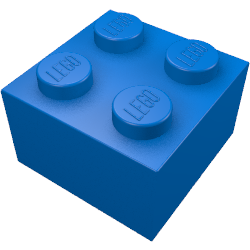
\includegraphics[width=0.3\textwidth,height=\textheight,keepaspectratio]{images/3003.png}
            \caption{Vyrenderovaná součástka z~ukázky kódu \ref{ukazka-soucastky-ldraw} \autocite{rebrickable:part:image:3003}\label{obrazek-ldraw-soucastka}}
        \end{figure}

    \subsubsection{Knihovna LDraw}\label{ldraw-knihovna}
    Knihovna \textbf{LDraw} poskytuje velké množství\footnote{V době psaní práce obsahuje knihovna 9 781 součástek} 3D modelů LEGO součástek ve formátu \textit{LDraw}.

    Součástky z~knihovny je možné obdržet jednotlivě z~adresy \\ \textit{http://www.ldraw.org/library/official/<filepath>} kde \textit{<filepath>} je cesta k~souboru v knihovně \textbf{LDraw}  \autocite{ldraw:download}. Další možností je obdržení kompletní knihovny v~podobě ZIP archivu. Struktura obsahu tohoto archivu je zobrazena na diagramu adresářové struktury \ref{ldraw-archiv}.

    \begin{dirfigure}%
        \dirtree{%
            .1 models\DTcomment{složka do které jsou ukládány vytvořené modely}.
            .1 p \DTcomment{primitiva používaná při tvorbě modelů}.
                .2 8.
                .2 48.
            .1 parts\DTcomment{kompletní součástky}.
                .2 *.dat\DTcomment{soubory součástek}.
                .2 s\DTcomment{často používáné společné části součásek}.
            .1 CAlicense.txt\DTcomment{licenční podmínky}.
            .1 CAreadme.txt\DTcomment{vysvětlení licenčních podmínek}.
            .1 LDConfig.ldr\DTcomment{definice barev}.
            .1 Readme.txt\DTcomment{popis obsahu archivu}.
            .1 mklist.exe\DTcomment{program MKList k~vytvoření seznamu součástek}.
            .1 mklist1\_6.zip\DTcomment{archiv se zdrojovým kódem programu MKList}.
        }
        \caption{Obsah archivu complete.zip}\label{ldraw-archiv}
    \end{dirfigure}

    Aby byla vytvořená součástka přidána do oficiální knihovny \textbf{LDraw}, musí projít schvalovacím procesem. V~tom je kontrolováno dodržení všech pravidel specifikace formátu \autocite{ldraw:file:specification} i další pravidla platná pro knihovnu \cite{ldraw:library:restrictions}.

    \subsubsection{Hlavička souboru}\label{ldraw-hlavicka}
        Každý \textit{LDraw} soubor, který se nachází v~knihovně, musí obsahovat hlavičku s~obsahem řídícím se pravidly \autocite{ldraw:header:specification}. V~hlavičce souboru jsou uložena metadata poskytující doplňující informace o~součástce. Mezi tyto informace mimo jiné patří:
        \begin{itemize}
            \item název,
            \item autor,
            \item licence,
            \item typ součástky,
            \item klíčová slova,
            \item kategorie.
        \end{itemize}
 
    \subsubsection{Typy prvků}\label{ldraw-typy-soucastek}
    V~knihovně se nachází prvky několika různých typů. Specifikace je v~tomto ohledu velmi rozsáhlá \autocite{ldraw:header:specification}\autocite{ldraw:sticker:specification}. Typ prvku je možné rozpoznat podle: 
    \begin{itemize}
        \item názvu (první řádek souboru \textit{LDraw}),
        \item META příkazů hlavičky,
        \item čísla (jméno souboru).
    \end{itemize}
    
    Po detailním prozkoumání většího množství prvků musím podotknout, že ne všechny soubory knihovny přesně odpovídají specifikaci. 

    Možné typy prvků:
    
    \begin{itemize}
        \item \textbf{Part:} Geometricky kompletní součástka.
        \item \textbf{Subpart:} Sám o~sobě nekompletní útvar.
        \item \textbf{Primitive:} Základní geometrický útvar vyskytující se v~mnoha součáskách.

        Pro více informací o primitivech a jejich kompletní seznam doporučuji \autocite{ldraw:primitives}.

        \item \textbf{Shortcut:} Součástka složená z~více kompletních součástek.

        Na obrázku \ref{obrazek-ldraw-shortcut} je možné vidět render součástky \textit{970c00} skládající (nahoře) se ze součástek \textit{3815}, \textit{3816}, \textit{3817} (dole).

        \item \textbf{Alias:} Soubor odkazující na jiné místo v~knihovně (například z~důvodu používání dvou růzých čísel pro stejný prvek společností LEGO). 
        
        Soubor typu \textit{Alias} typicky obsahuje pouze jeden příkaz typu \text{1}. Náhled souboru typu \textit{Alias} je k~vidění v~ukázce kódu \ref{ukazka-alias}.

        \item \textbf{Physical\_Colour:} Soubor odkazující na jiné místo v~knihovně a navíc určující barvu.
        \item \textbf{Sticker:} Potisk.
        \item \textbf{Patterned:} Součáska s~potiskem (viz. obrázek \ref{obrazek-ldraw-patterned}).
    \end{itemize}
   
    \begin{figure}[htbp]
        \centering
        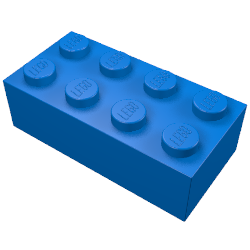
\includegraphics[width=0.3\textwidth,height=\textheight,keepaspectratio]{images/3001.png}
        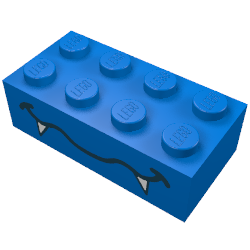
\includegraphics[width=0.3\textwidth,height=\textheight,keepaspectratio]{images/3001p0b.png}
        \caption{Ukázka dílu typu \textit{Patterned} \autocite{rebrickable:part:image:3001}\autocite{rebrickable:part:image:3001p0b}\label{obrazek-ldraw-patterned}}
        %TODO - reference
    \end{figure}

      \begin{listing}[htbp]
        \begin{minted}[bgcolor=codebg]{text}
0 ~Moved to 6141
0 Name: 4073.dat
0 Author: [PTadmin]
0 !LDRAW_ORG Part Alias UPDATE 2015-01
0 !LICENSE Redistributable under CCAL version 2.0 : see CAreadme.txt

0 BFC CERTIFY CCW

0 !HISTORY 2015-10-11 [PTadmin] Official Update 2015-01

0 // Plate  1 x  1 Round

1 16 0 0 0 1 0 0 0 1 0 0 0 1 6141.dat
        \end{minted}
        \caption{Ukázka souboru typu \textit{Alias} \autocite{ldraw:model:alias}\label{ukazka-alias}}
    \end{listing}

    \begin{figure}[htbp]
        \centering
        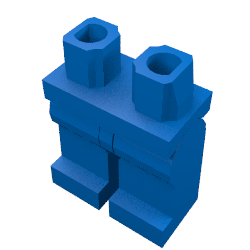
\includegraphics[width=0.4\textwidth,height=\textheight,keepaspectratio]{images/3815c01.png}
        \\
        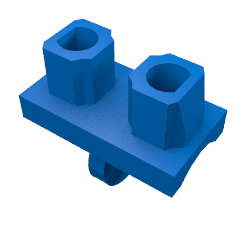
\includegraphics[width=0.3\textwidth,height=\textheight,keepaspectratio]{images/3815.png}
        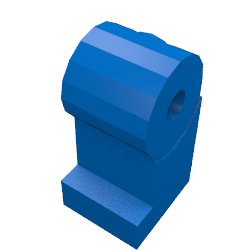
\includegraphics[width=0.3\textwidth,height=\textheight,keepaspectratio]{images/3816.png}
        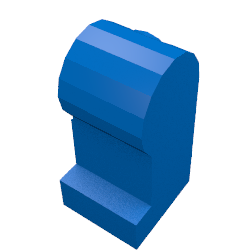
\includegraphics[width=0.3\textwidth,height=\textheight,keepaspectratio]{images/3817.png}
        \caption{Ukázka dílu typu \textit{Shortcut} \autocite{rebrickable:part:image:970c00}\autocite{rebrickable:part:image:3815}\autocite{rebrickable:part:image:3816}\autocite{rebrickable:part:image:3817}\label{obrazek-ldraw-shortcut}}
    \end{figure}

    Pravidla pojmenovávání jednotlivých souborů s~ohledem na jejich typ jsou znázorněna v~tabulce \ref{tabulka-ldraw-cislovani}.

    \begin{table}[th!]
    \centering
        \caption{Shrnutí pravidel pro číslování součástek \autocite{ldraw:numbering:faq}}
        \label{tabulka-ldraw-cislovani}
        \begin{tabularx}{\textwidth}{@{}rX@{}}
        \toprule
        Vzor pojmenovávání & Typ prvku
        \\ \midrule
        nnn, nnnn, nnnnn & \textit{Part}
        \\
        <number>Cnn & \textit{Shortcut}
        \\
        <number>Dnn & kombinace \textit{Part} a \textit{Sticker}
        \\
        <number>Pxx & \textit{Patterned} 
        \\
        s/<number> & \textit{Subpart} (umístěná ve složce parts/s)
        \\
        <number>a & Novější verze součásky <number>
         \\
        \bottomrule
        \multicolumn{2}{l}{n = číslice, x = číslice/písmeno, a = písmeno}
        \\
        \multicolumn{2}{l}{<number> = kompletní pojmenovávání jiného prvku}
        \end{tabularx}
    \end{table}

    \subsubsection{Licence}\label{ldraw-licence}
    Všechny součástky zahrnuté do oficiální knihovny \textbf{LDraw} jsou vydány pod licencí \gls{CC-BY} \autocite{CC-BY}. Ta umožňuje úpravu i sdílení díla za předpokladu dodržení podmínky o~uvedení autora, licence a označení případných provedených změn.

    % \subsubsection{Závěr}\label{ldraw-zaver}
    %TODO
    
    %  Součástky navíc obsahují doplňující informace, pomocí kterých je možné je třídit a vyhledávat. 
\subsection{Brickset}\label{reserse-brickset}
  Brickset je populární webová aplikace poskytující detailní informace a novinky o~stavebnicích LEGO. Má rozsáhlou základnu aktivních uživatelů\footnote{Brickset má více než 150 000 registrovaných uživateů a v~průměru 20 000 aktivních uživatelů každý měsíc. \autocite{brickset:infographic}} a sama o~sobě prohlašuje, že je primárním zdrojem informací o~LEGO stavebnicích na internetu \autocite{brickset:about}.

  \subsubsection*{Poskytovaná data}
  Data z~databáze Brickset jsou dostupná přes veřejné \gls{API}. Přes \gls{API} je možné obdržet informace týkající se stavebnic, instrukce k~jejich postavení, recenze a obrázky stavebnic. Dále je přes Brickset \gls{API} možné spravovat uživatelské sbírky stavebnic. 

  Přestože webové stánky Brickset umožňují i prohlížení inventářů jednotlivých stavebnic, Brickset nemá oprávnění k~jejich sdílení přes své   \gls{API} a ve své dokumentaci \autocite{brickset:api} odkazuje k~využítí \gls{API} webové stránky Rebrickable.com. 

  \subsubsection*{API}
  Podrobná specifikace \gls{API} s~výčtem dostupných metod je na \autocite{brickset:api}. Brickset \gls{API} je implementováno jako služba postavená nad protokolem \gls{SOAP}. 

  \subsubsection*{Závěr}
  Pro účely vytvářené aplikace není využití samotných dat poskytovaných přes \gls{API} Brickset dostačující. Bude tedy nutné využít další zdroje poskytující informace o~inventářích stavebnic. \gls{API} služby Brickset bude využito pouze k~obdržení popisu stavebnic, obrázků, instrukcí a recenzí.
\subsection{Rebrickable}\label{reserse-rebrickable}
  Rebrickable \autocite{rebrickable:homepage} je webová aplikace sloužící ke správě sbírek LEGO součástek a stavebnic. Umožňuje uživateli prohlížení rozsáhlé databáze obsahující více než 11 500 oficiálních stavebnic a více než 25 000 unikátních součástek prodávaných společností LEGO od roku 1950 po současnost \autocite{rebrickable:about}. 

  \subsubsection*{Poskytovaná data}  
  Rebrickable svou databázi zpřístupňuje dvěma způsoby. Jedním způsobem je pravidelný (měsíční) výpis z~databáze formou tabulek ve formátu \textit{\gls{CSV}}. Druhou možností je získávání dat přes veřejné \gls{API}. Struktura tabulek \textit{\gls{CSV}}, které jsou ke stažení ze stránek \autocite{rebrickable:download} je znázorněna na obrázku \emph{\ref{diagram-rebrickable}}.

  \subsubsection*{Číslování součástek}
  Velkou výhodou použití dat služby Rebrickable je systém číslování součástek, který vychází z~číslování u~knihovny LDraw \autocite{rebrickable:faq}. To ušetří velké množství práce při mapování součástek z~databáze Rebrickable na součástky knihovny LDraw. 
  
  \subsubsection*{Licence}
  Data aplikace jsou veřejně dostupná pro jakékoliv účely, včetně komerčních. Autoři aplikace pouze žádají o~zveřejnění prohlášení o~původu dat. \autocite{rebrickable:terms}
  
  \begin{figure}[htbp]
    \centering
    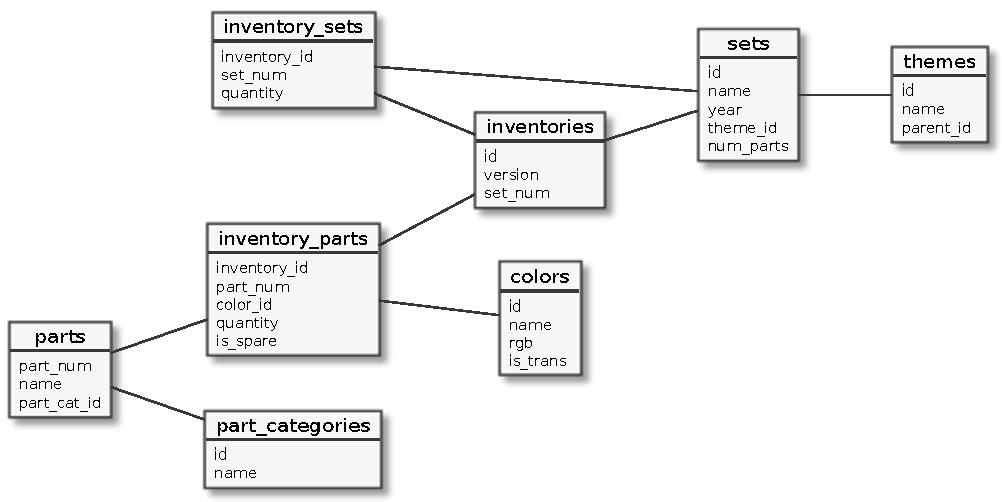
\includegraphics[width=\textwidth,height=\textheight,keepaspectratio]{pdfs/rebrickable_schema}
    \caption{Diagram schématu, Rebrickable \autocite{rebrickable:download}\label{diagram-rebrickable}}
  \end{figure}

  \subsubsection*{Závěr}
  Pro získání dat o~inventářích jednotlivých stavebnic bude využita databáze služby Rebrickable ve formě \textit{\gls{CSV}} tabulek. Využití kompletních dat je pro účely aplikace optimálním řešením. Na rozdíl od varianty dynamického získávání dat přes \gls{API} umožňuje předem připravené namapování součástek na 3D modely a celkově rychlejší přístup k~datům.
\subsection{Další zdroje dat}
V~rámci rešerše jsem se seznamoval i s~dalšími službami, které poskytují data o~inventářích stavebnic LEGO – Bricklink \autocite{bricklink} a BrickOwl \autocite{brickowl}. Obě služby poskytují také svá data pomocí \gls{API}, nevychází však u~číslování součástek ze systému LDraw a tak by párování 3D modelů a součástek bylo o~poznání složitější. 

\section{Převod formátu}
S~ohledem na požadavek na zajištění převodu formátu LDraw je v~této sekci nejprve představen formát \textit{\gls{STL}} nejčastěji využívaný k~3D tisku \autocite{3DAddFab}. Následně jsou představena možná řešení samotného převodu. Nakonec jsou představeny nástroje pro vykreslení souborů \textit{STL}.

\subsection{STL}
Souborový formát \textit{\gls{STL}}, byl vyvinut firmou 3D Systems. Soubor popisuje třírozměrnou povrchovou geometrii modelu a je nejčastěji používaným souborovým formátem pro potřeby 3D tisku. \autocite{3DAddFab}

\subsection{LDView}\label{podsekce-ldview}
\begin{figure}[htbp]
        \centering
        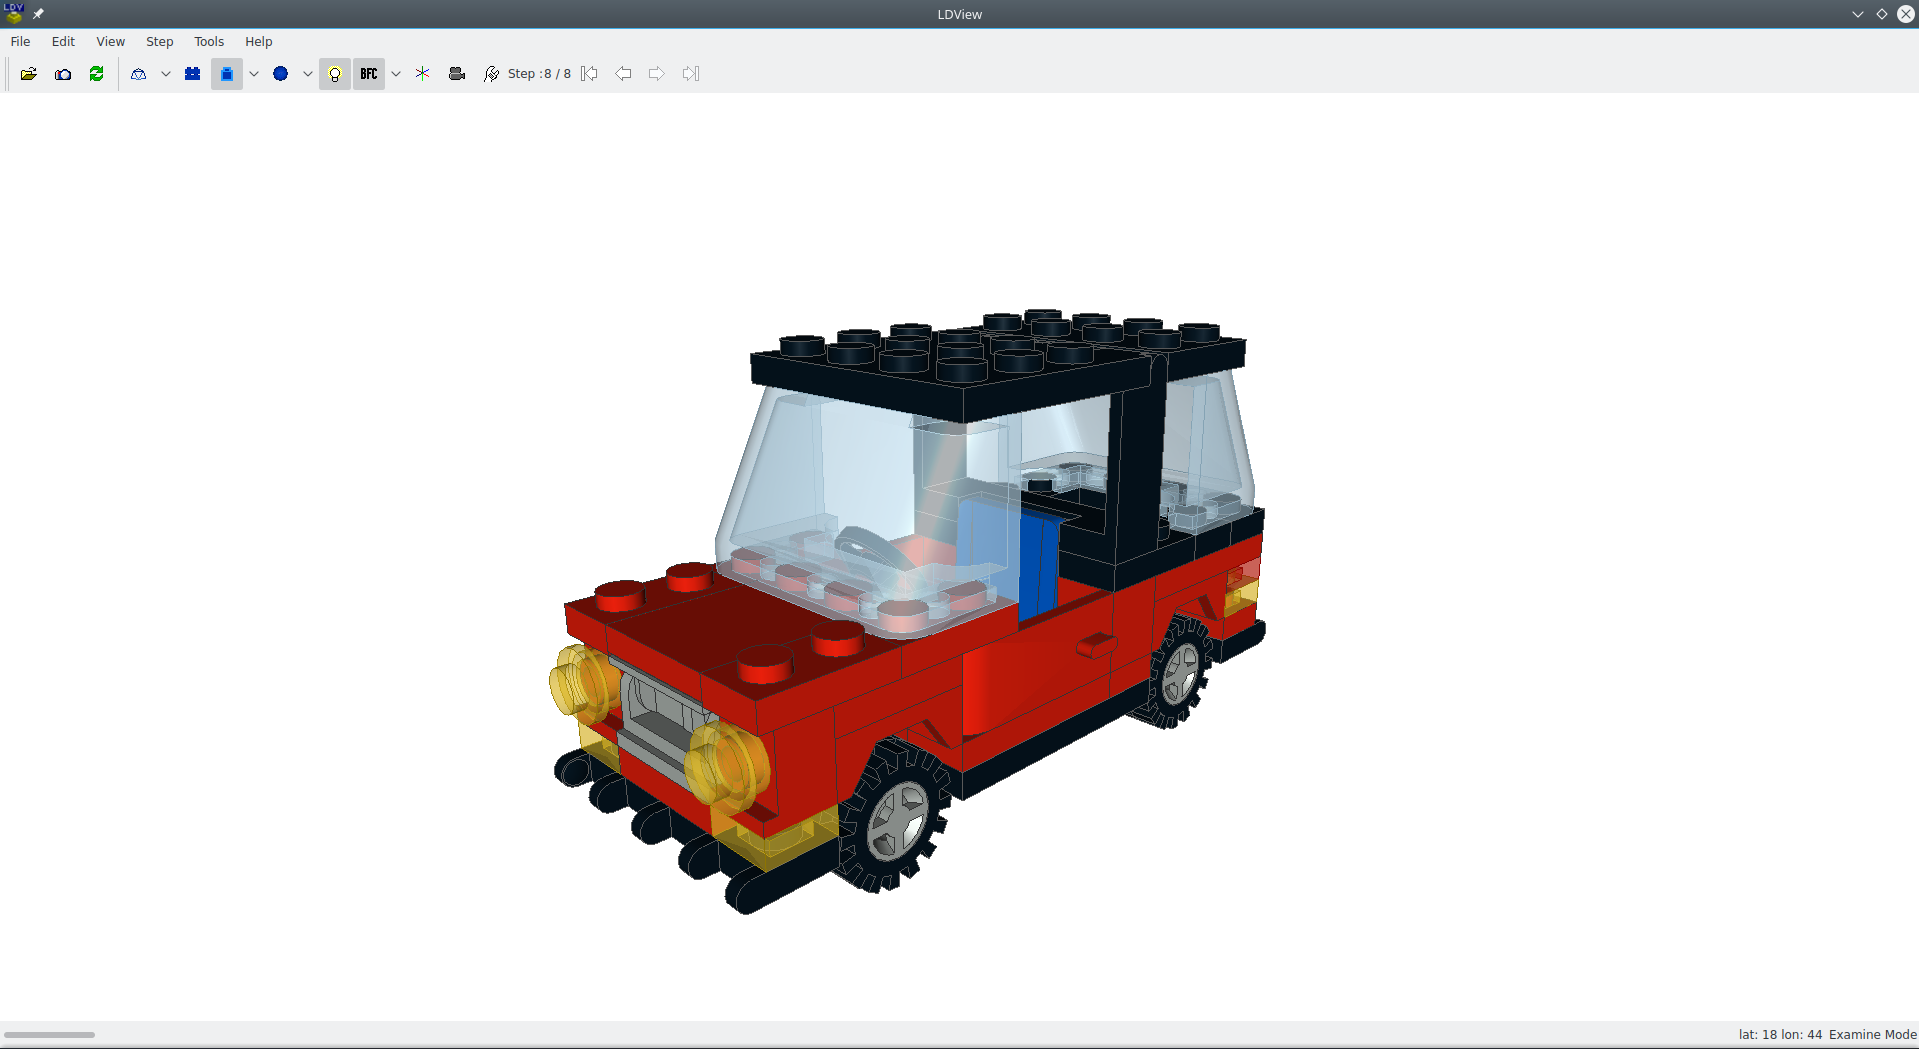
\includegraphics[width=\textwidth,height=\textheight,keepaspectratio]{images/ldview.png}
        \caption{Snímek obrazovky programu LDView}
\end{figure}

LDView je 3D prohlížeč modelů a součástek ve formátu LDraw, představeného v~sekci \emph{\nameref{ldraw-format}} na straně \emph{\pageref{ldraw-format}}. Program je veřejně dostupný pod licencí \gls{GPLv2} \autocite{GPLv2}.

Mezi jedny z~funkcí programu patří: 
\begin{itemize}
    \item schopnost exportovat LDraw modely do formátů \textit{POV-Ray}, \textit{3DS} nebo \textit{STL},
    \item schopnost pořizovat snímek aktuálního pohledu.
\end{itemize}

Program je dostupný jak ve verzi s~grafickým prostředím, tak v~konzolové verzi využitelné například na systémech bez grafického prostředí.

Pro více informací o~programu a jeho dostupných funkcích doporučuji \autocite{ldview}.

\subsubsection*{Převod formátu}

Převod formátu LDraw do jiných formátů pomocí programu LDView je velmi jednoduchý. V~ukázce \emph{\ref{priklad-ldview}} je příklad použití konzolové verze programu. 

Při konzultaci s~vedoucím bylo odhaleno, že převedené součástky mají 10krát menší meřítko a jsou o~90° otočené kolem osy X. Formát \textit{\gls{STL}} dle specifikace \autocite{stl:specification} nemá jednotku a není definováno, která osa ukazuje směrem vzhůru. Při \gls{FDM} 3D tisku je však praxí, že se předpokládá jenotka mm a osa Z~směřující vzhůru. Z~tohoto důvodu je vhodné provést korekci souborů \textit{STL}.

Oprava těchto chyb ve zdrojovém kódu programu by stála velké množství práce a náročné zorientování se v~cizím kódu. Proto jsem se rozhodl opravu měřítka a natočení modelu provést pomocí nástroje ADMesh. 

 \begin{listing}[htbp]
        \begin{minted}{bash}
$ ldview ./ldraw/parts/3003.dat -LDrawDir=./ldraw -ExportFile=3003.stl 
        \end{minted}
    \caption{Příklad použití programu LDView \label{priklad-ldview}}
\end{listing}



\subsection{ADMesh}
ADMesh \autocite{ADMesh} je open-source program umožňující provádět operace nad soubory ve formátu \gls{STL}. Jedná se o program bez grafického rozhraní spouštěný z příkazové řádky. 

Funkce:
\begin{itemize}
    \item kontrolování závad (chybné normálové vektory, neuzavřené stěny) i jejich automatická oprava,
    \item rotace modelu,
    \item traslace,
    \item změna velikosti,
    \item čtení a zápis binárních i textových \gls{STL} souborů.
\end{itemize}
\section{Vykreslení modelů}\label{reserse-vykresleni}
Pro možnost poskytnout uživatelsky přívětivé a přehledné prostředí aplikace je nepochybně nutné mít možnost zobrazit součástky v~podobě statického obrázku. Obrázek většiny součástek z~knihovny LDraw je volně k~dispozici ke stažení z~webových stránek již představené služby Rebrickable \autocite{rebrickable:download}. Pro zbytek součástek je však nutné obrázek vyrenderovat. 

Nejjednodušší možností pro vyrenderování obrázků součástek je využití již představeného programu LDView, který bude v~aplikaci využíván. Program umožňuje jako jednu ze svých funkcí i vykreslení aktuálního pohledu. Tato možnost se však ukázala jako velmi nespolehlivá (v~závislosti na operačním systému, na kterém je program volán).

Proto jsem se rozhodl využít jiné nástroje k~vyrenderování obrázků součástek a to sice programy stl2pov \autocite{stl2pov} a POV-Ray \autocite{povray}.

\subsection{POV-Ray}
Dle \autocite{root:povray} je POV-Ray nástroj pro vykreslování trojrozměrných scén s~důrazem na co nejvyšší kvalitu výsledku. Celá scéna je popsána v~textovém souboru, který svou podobou připomíná jazyk C. POV-Ray takto popsanou scénu přečte, provede vykreslení a výsledek uloží ve formě rastrového obrázku. Podobu příkazu pro vykreslení scény na pozadí je možné vidět v~ukázce kódu \emph{\ref{priklad-povray}}. 

\begin{listing}[htbp]
        \begin{minted}{console}
$ povray +W900 +H600 +FN -D +I"input.pov" +O"output.png" 
        \end{minted}
    \caption{Příklad použití programu POV-Ray \label{priklad-povray}}
\end{listing}

\subsection{Stl2pov}
Stl2pov je program umožňující převod \textit{\gls{STL}} souboru na POV-ray objekt, který je možné použít do specifikace POV-ray scény k~vykreslení.  


\chapter{Požadavky}\label{kapitola-pozadavky}
V~této sekci jsou shrnuty požadavky kladené na vytvářenou aplikaci specifikované v~zadání této práce. Požadavky jsou rozděleny na funkční a nefunkční.

\subsection{Funkční požadavky}

\begin{enumerate}[label=FP-\arabic*]
    \item \label{fp:model:search} \textbf{Procházení, vyhledávání a prohlížení součástek a stavebnic}

    Aplikace musí umožňovat procházení, vyhledávání a prohlížení součástek z~knihovny LDraw a stavebnic z~databáze Brickset. 

    \item \label{fp:model:download} \textbf{Stažení 3D modelů}

    3D modely součástek musí být možno stáhnout samostatně i v~sadách modelů obsažených v~jednotlivých stavebnicích. Stavebnice navíc musí být možno stáhnout i ve verzi roztříděné podle barev součástek.

    \item \label{fp:model:prevod} \textbf{Zajištění převodu formátu LDraw na formát vhodný pro 3D tisk}

    Převod formátu bude zajištěn využitím vhodné existující implementace konverze. 

    \item \label{fp:model:3Dview} \textbf{Interaktivní prohlížení součástek ve 3D náhledu}

    Aplikace musí umožňovat interaktivní prohlížení součástek ve 3D náhledu.

    \item \label{fp:model:update} \textbf{Automatická aktualizace databáze LDraw}

    Databázi součástek z~knihovny musí být možné automaticky aktualizovat.

\end{enumerate}

\subsection{Nefunkční požadavky}

\begin{enumerate}[label=NP-\arabic*,resume]
    \item \label{np:opensource} \textbf{Open-source kód}

    Zdrojový kód aplikace musí být vydán pod open-source licencí.

    \item \label{np:webgl} \textbf{Využití WebGL pro 3D náhled součástek}
    
    K~interaktivnímu prohlížení součástek ve 3D náhledu musí být využito \gls{WebGL}.

    \item \label{np:structure} \textbf{Dobře strukturovaný, řádně otestovaný, vhodně okomentovaný a dokumentovaný zdrojový kód}
    \item \label{np:english} \textbf{Komentáře i dokumentace v~anglickém jazyce}
\end{enumerate}
\chapter{Návrh}\label{kapitola-navrh}
Důležitou součástí každého vývoje je návrhová fáze. V~této fázi jsou využity znalosti získané během analytické a rešeršní části práce. Návrh je později využit při implementační fázi vývoje. Tato kapitola se nejprve zabývá výběrem vhodných technologií pro implementační část práce.
Dále se zabývá návrhem architektury aplikace a návrhem uživatelského rozhraní.

\section{Technologie}
Jednou ze základních otázek při tvorbě webové aplikace je volba technologií, které budou při implementaci využity. Od volby se odvíjí jak návrh, tak implementace samotná. 

\subsection{PHP}
Pro tvorbu webové aplikace jsem se rozhodl využít programovacího jazyka \gls{PHP}. Jedním z~hlavních kritérií zohledněných při výběru technologie byla jistá předchozí zkušenost s~programovacím jazykem PHP, který patří mezi nejpoužívanější technologie pro tvorbu webových aplikací. V~současné době je v~jazyce PHP napsáno více než 82 \% webových stránek se skriptováním na straně serveru \autocite{web:statistics}. Vzhledem k~vysoké rozšířenosti je o~jazyce PHP dostupné velké množství informací, které usnadňují vývoj. 

\subsection{Framework Symfony 3}
Po provedení průzkumu mezi PHP frameworky jsem se rozhodl svou práci vyvíjet s~využitím frameworku Symfony 3. Hlavním důvodem pro výběr Symfony byla nativní podpora konzolových příkazů \autocite{symfony:console}, kvalitně zpracovaná dokumentace a využití knihovny Doctrine \gls{ORM} \autocite{symfony:doctrine}.
% \section{Návrh architektury}


% \subsection{Vrstvy aplikace}
% Aplikace se skládá ze tří vrstev podle architektury \gls{MVC}, typické pro PHP framework Symfony. 
\section{Doménový model}
Doménový model (na obrázku \emph{\ref{diagram-domenovy}} a \emph{\ref{diagram-domenovy-brickset}}) popisuje strukturu dat a vazby mezi jednotlivými entitami. Je důležitý pro učinění rozhodnutí jaké objekty a jejich vztahy bude nutné v~aplikaci uchovávat. 

Při vytváření doménového modelu je vycházeno ze tří zdrojů dat, které jsou stanoveny v~rešeršní části práce. Z~hlediska domény je tedy vhodné rozdělit entity do balíčků podle zdroje, ze kterého pochází. Využité zdroje dat jsou: 
\begin{itemize}
  \item knihovna LDraw,
  \item Rebrickable,
  \item Brickset.
\end{itemize}

Pro větší přehlednost jsem doménový model rozdělil na dva diagramy. Diagram na obrázku \emph{\ref{diagram-domenovy}} popisuje lokálně ukládaná data knihovny LDraw a služby Rebrickable. Diagram na obrázku \emph{\ref{diagram-domenovy-brickset}} data dostupná přes API Brickset. 

\begin{figure}[htbp]
    \centering
    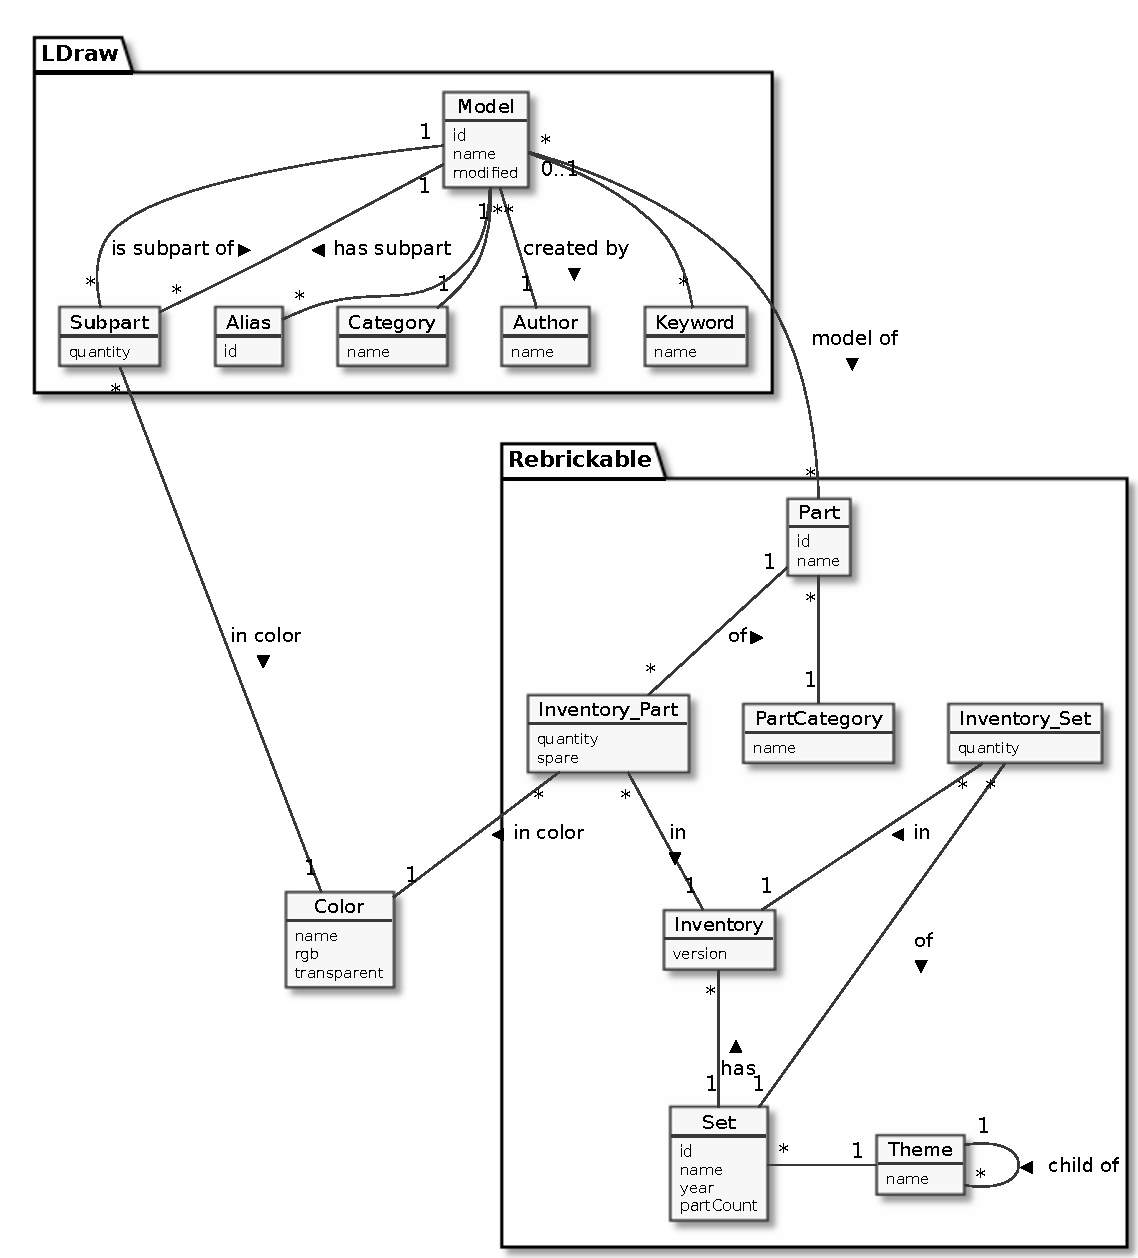
\includegraphics[width=\textwidth,height=\textheight,keepaspectratio]{pdfs/domain_ldraw_rebrickable}
    \caption{Doménový model: LDraw a Rebrickable\label{diagram-domenovy}}
  \end{figure}

\subsection{LDraw}
První balíček obsahuje entity týkající se součástek z~knihovny LDraw.

\subsubsection*{Model}
  Entita \textit{Model} (tabulka \emph{\ref{table:entity:model}}) reprezentuje jednu součástku z~knihovny LDraw. Atributy entity vychází z~dat obsažených v~jednotlivých souborech knihovny a ze specifikace hlavičky, která byla představena v~podsekci \emph{\nameref{ldraw-hlavicka}} sekce \emph{\ref{reserse-ldraw}}.
    
  U~každého \textit{Modelu} musí být evidován jeho autor z~důvodu možnosti dodržení licence \gls{CC-BY} \cite{CC-BY}, pod kterou jsou zveřejněny všechny součástky v~oficiální knihovně LDraw. 
  
  \begin{table}[th!]
  \centering
  \caption{Přehled atributů entity \textit{Model}}
  \label{table:entity:model}
  \begin{tabularx}{\textwidth}{@{}rX@{}}
  \toprule
  Atribut & Popis
  \\ 
  \midrule
  id: & Unikátní textový identifikátor modelu
  \\
  name: & Jméno modelu 
  \\
  modified: & Datum poslední úpravy modelu 
  \\
  partCount: & Počet součástek ve stavebnici
  \\
  path: & Cesta k~souboru 3D modelu na serveru
  \\
  \bottomrule
  \end{tabularx}
  \end{table}

\subsubsection*{Author}
Entita \textit{Author} reprezentuje autora, který svými modely přispívá do knihovny LDraw. Aby mohl být model zahrnut do oficiální knihovny, musí být autor registrován a projevit souhlas s~Dohodou přispěvatelů Ldraw.org \autocite{ldraw:agreement}.
  
\subsubsection*{Alias}
Entita \textit{Alias} reprezentuje alternativní identifikátor modelu, na který má vazbu. 

Uchování alternativních identifikátorů modelů slouží ke sjednocení tvarově identických součástek. Uchovávání každé součástky by z~hlediska 3D tisku nemělo žádný význam, protože jejich rozdíly (například potisk) zaniknou okamžikem převodu do formátu \textit{STL}.

\subsubsection*{Subpart}
Protože formát LDraw umožňuje i vytváření součástek typu \textit{Shortcut}, které jsou definovány v~podsekci \emph{\nameref{ldraw-typy-soucastek}} sekce \emph{\ref{reserse-ldraw}}, je nutné mít možnost uchovat informaci o~vztahu mezi jednotlivými modely. Toto je umožněno entitou \textit{Subpart}. 

Entita \textit{Subpart} kromě vazeb na \textit{Model} obsahuje atribut specifikující četnost výskytu podsoučástky a vazbu na entitu \textit{Color}, která specifikuje barvu. 

\subsubsection*{Category}
Každý model je zařazen do kategorie, která je určena v~hlavičce souboru.

\subsubsection*{Keyword}
K~možnosti vyhledávání v~knihovně LDraw mohou součástky a podsoučástky definovat klíčová slova.

\subsection{Rebrickable}
Druhý balíček sdružuje entity ze služby Rebrickable, která poskytuje inventáře součástek a stavebnic.

\subsubsection*{Set}
Entita \textit{Set} reprezentuje jednu stavebnici LEGO. Každá stavebnice má své unikátní id určené přímo společností LEGO. 

\subsubsection*{Part}
Entita \textit{Part} reprezentuje jednu unikátní součásku LEGO z~databáze Rebrickable.

\subsubsection*{Inventory}
Stavebnice může být během času vydána v~novější verzi, ve které je například vyměněna pouze jedna součástka. To vede k~potřebě zvláštní entity \textit{Inventory}, která reprezentuje tyto verze inventářů. 

\subsubsection*{Inventory\_Part} 
Součástky se ve stavebnicích mohou vyskytovat v~různých barevných provedeních. Dále je běžné, že stavebnice LEGO obsahují některé součástky navíc, které nejsou nezbytné k~jejich sestavení. Proto je v~nutná entita \textit{Inventory\_Part}, která umožňuje zaznamenání tohoto vztahu mezi součástkou a inventářem, včetně informace o~počtu, barvě a typu součástky.

\subsubsection*{Inventory\_Set}
Stavebnice se nemusejí skládat pouze ze součástek, ale mohou sdružovat i větší množství jiných stavebnic. Proto je nutná entita \textit{Inventory\_Set}, která reprezentuje tento vztah mezi stavebnicí a inventářem.

\subsubsection*{Theme}
Každá stavebnice náleží do série. Série je reprezentována entitou \textit{Theme}. Série může být zároveň podřazena jiné sérii. Zpravidla je zanoření maximálně tři úrovně hluboké.

\subsubsection*{Color} 
Entita \textit{Color} (tabulka \emph{\ref{table:entity:color}}) je společná pro oba balíčky. To je dáno faktem, že Rebrickable se svými daty vychází právě z~knihovny LDraw, jak bylo zmíněno v~sekci \emph{\ref{reserse-rebrickable}}.

\begin{table}[th!]
  \centering
  \caption{Přehled atributů entity \textit{Color}}
  \label{table:entity:color}
  \begin{tabularx}{\textwidth}{@{}rX@{}}
  \toprule
  Atribut & Popis
  \\ \midrule
  id: & Unikátní LDraw id barvy \autocite{ldraw:colors}
  \\
  name: & Jméno barvy
  \\
  rgb: & Hexadecimální \gls{RGB} kód barvy 
  \\
  transparent: & Indikátor o~transparentnosti barvy
  \\
  \bottomrule
  \end{tabularx}
\end{table}

\subsection{Brickset}
Třetí balíček popisuje strukturu dat dostupných přes Brickset \gls{API}.   

\begin{figure}[htbp]
    \centering
    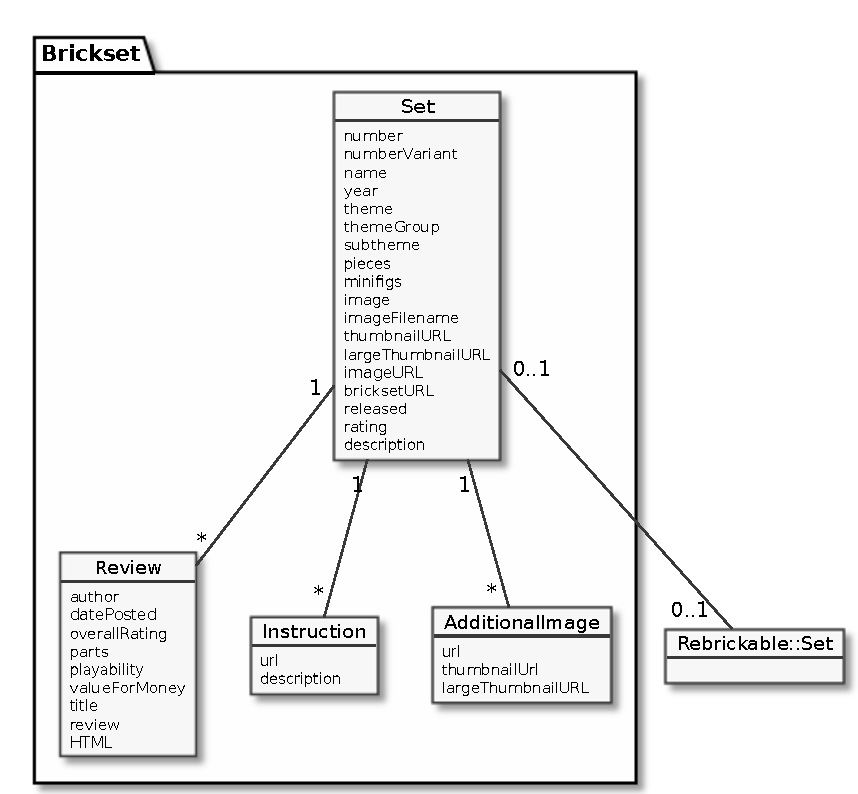
\includegraphics[width=\textwidth,height=\textheight,keepaspectratio]{pdfs/domain_brickset}
    \caption{Doménový model: Brickset \label{diagram-domenovy-brickset}}
\end{figure}

\subsubsection*{Set}
Entita \textit{Set} reprezentuje jednu stavebnici LEGO. Tato entita odpovídá právě jedné nebo žádné entitě \textit{Set} z~balíků Rebrickable.  

\subsubsection*{Review}
Brickset umožňuje uživatelům vytvářet recenze na stavebnice. Tyto recenze jsou reprezentovány entitou \textit{Review}. Recenze kromě textového popisu obsahuje i číselné hodnocení hlavních kritérií, znázorněných v~diagramu.

\subsubsection*{Instruction} 
Instrukce k~postavení stavebnice je reprezentována entitou \textit{Instruction}.

\subsubsection*{AdditionalImage} 
Entita \textit{AdditionalImage} reprezentuje jeden obrázek stavebnice. Obrázky jsou dostupné kromě původní velikosti i v~podobě miniatur.



\section{Uživatelské rozhraní}

\subsection{Domovská stránka}
Návrh domovské stránky (obrázek \emph{\ref{wireframe-hlavni}}) je velmi minimalistický. Stránka slouží pouze k~seznámení uživatele s~významem aplikace a k~navigaci na další stránky pomocí dvou velkých bloků umístěných pod úvodní fotografií. V pravém horním rohu se nachází vyhledávací pole, které umožňuje uživateli rychlou navigaci na součástky a stavebnice.

\begin{figure}[htbp]
    \centering
    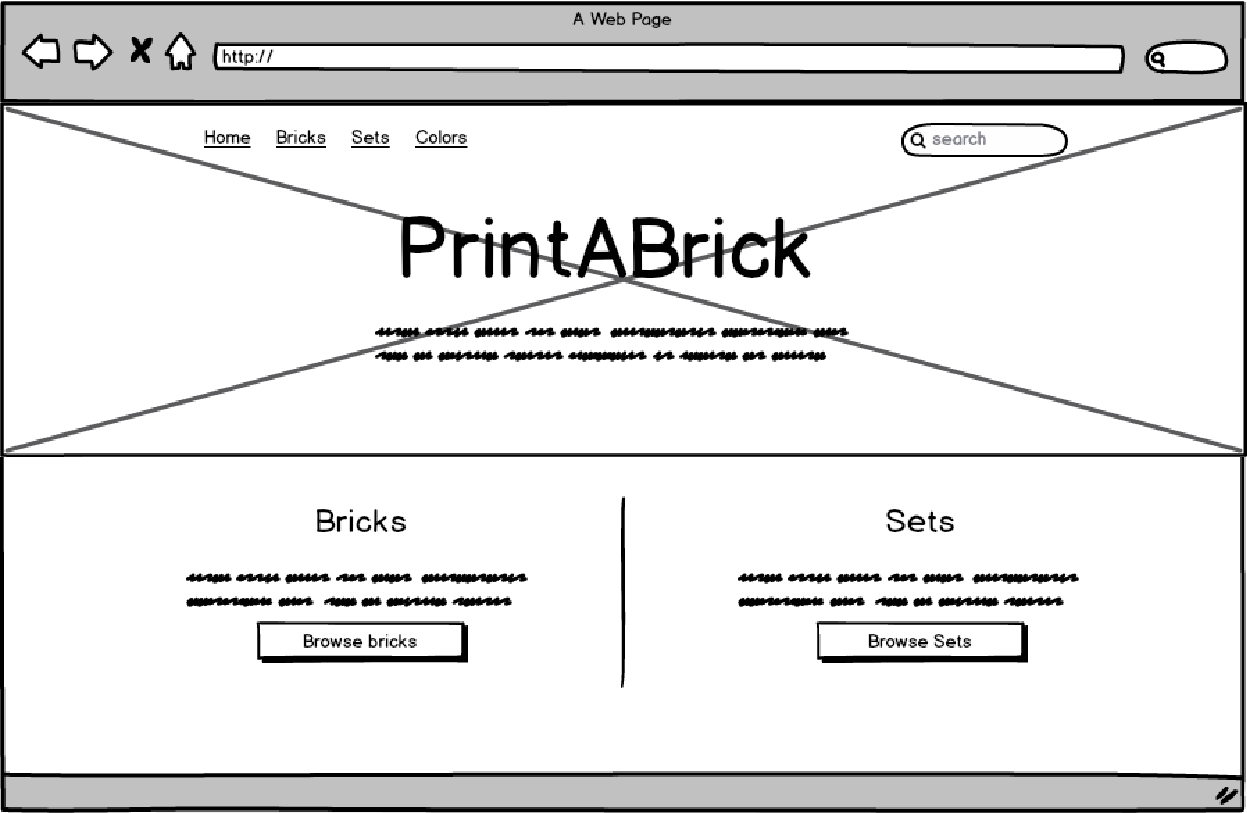
\includegraphics[width=\textwidth,height=\textheight,keepaspectratio]{pdfs/wireframe_home.pdf}
    \caption{Návrh hlavní stránky}\label{wireframe-hlavni}
\end{figure}


\subsection{Výpis stavebnic}
Na obrázku \emph{\ref{wireframe-stavebnice-seznam}} je možné vidět návrh stránky výpisu stavebnic. Tento výpis je stránkovaný a je možné ho řadit podle hlavních atributů stavebnic. Uživatel může specifikovat kritéria filtrování v~levém sloupečku. Sloupeček obsahuje textové pole pro zadání vyhledávaného výrazu, výběr kategorie a posuvníky určující počet součástek a rok vydání stavebnice.

Výpis stavebnic je zobrazen v~mřížce. Každý blok reprezentující stavebnici obsahuje obrázek a hlavní atributy, které mohou být uživateli nápomocné při výběru.

\begin{figure}[htbp]
    \centering
    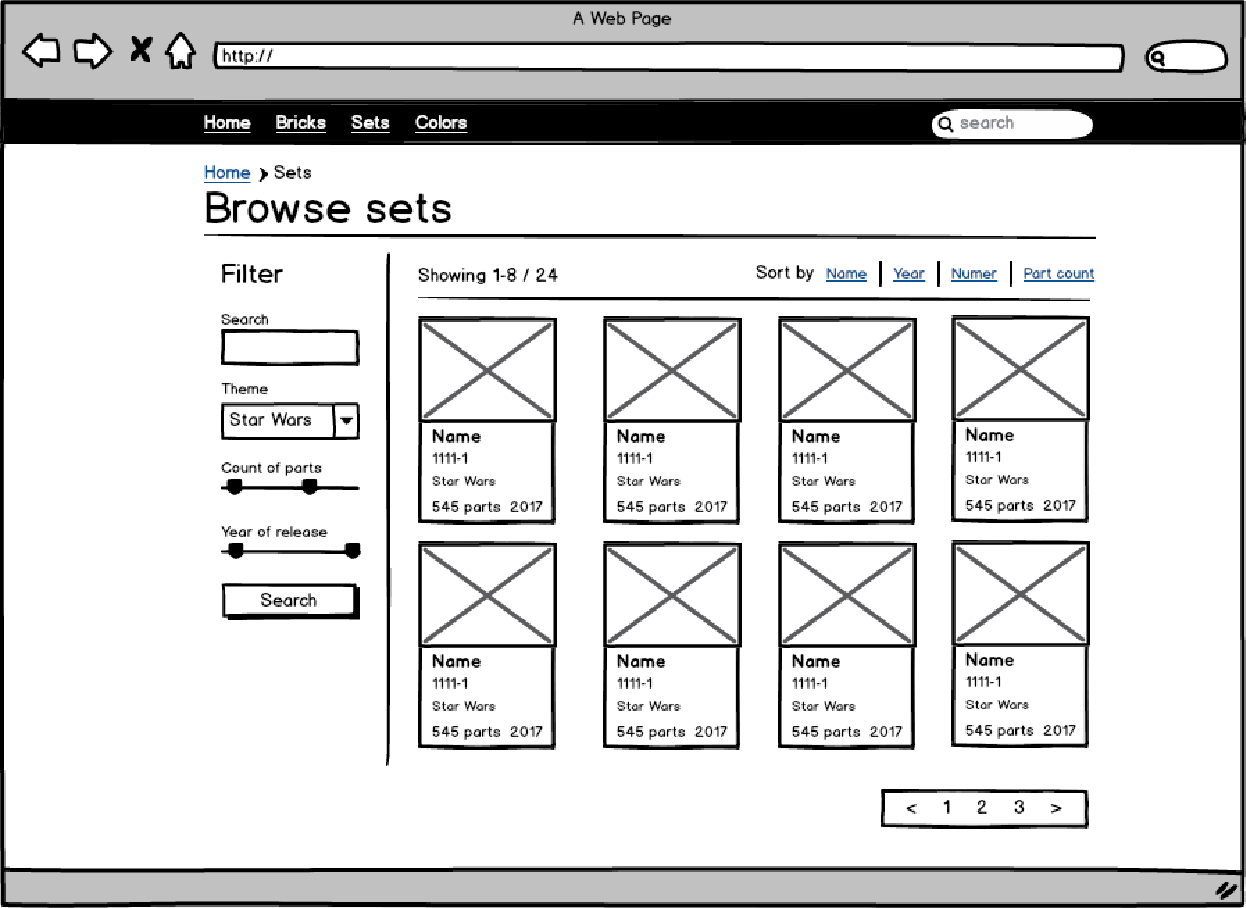
\includegraphics[width=\textwidth,height=\textheight,keepaspectratio]{pdfs/wireframe_sets.pdf}
    \caption{Návrh stránky výpisu stavebnic}\label{wireframe-stavebnice-seznam}
\end{figure}

\subsection{Výpis součástek}
Stránka výpisu součástek (obrázek \emph{\ref{wireframe-soucaska-seznam}}) je rozložením prvků navržena stejně jako stránka výpisu stavebnic. 

\begin{figure}[htbp]
    \centering
    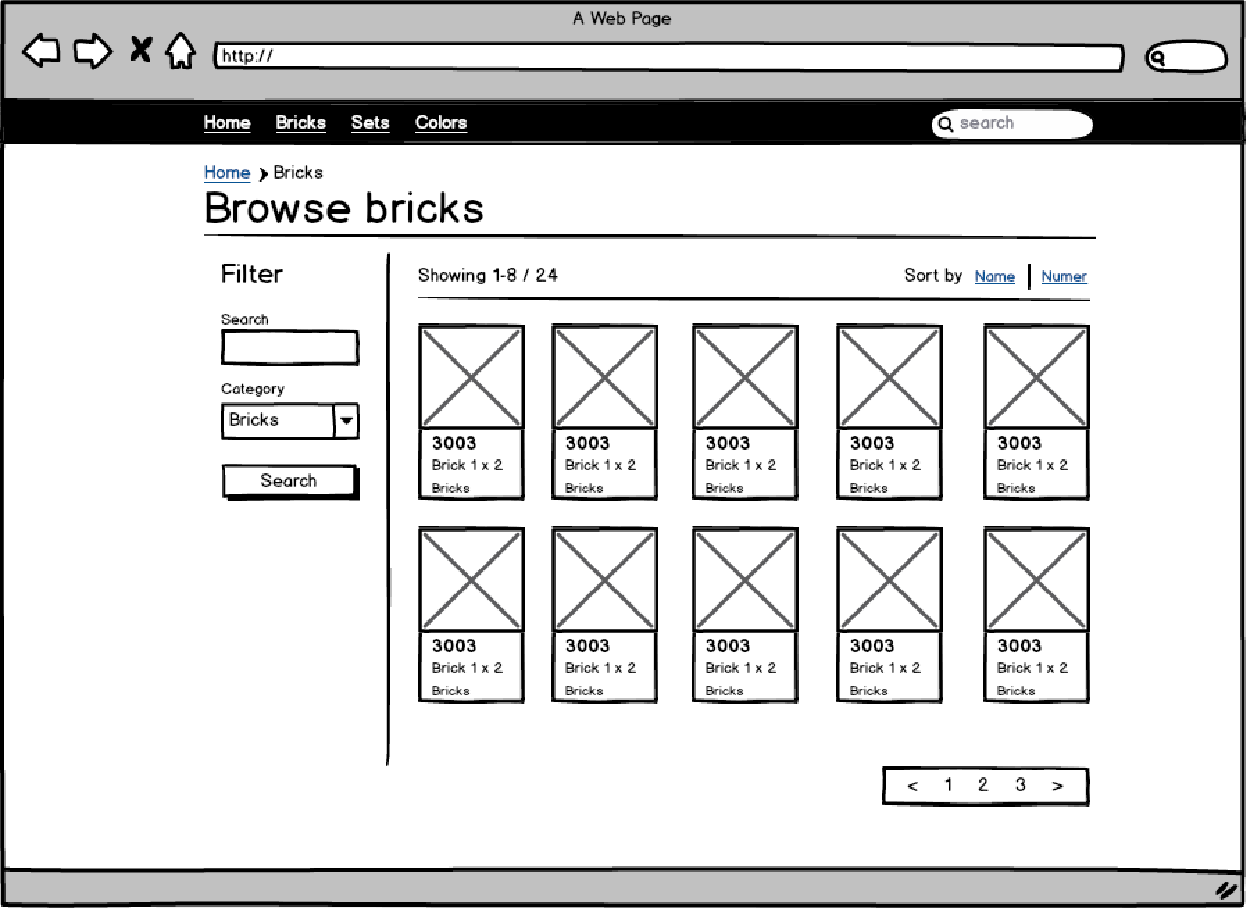
\includegraphics[width=\textwidth,height=\textheight,keepaspectratio]{pdfs/wireframe_bricks.pdf}
    \caption{Návrh stránky výpisu součástek}\label{wireframe-soucaska-seznam}
\end{figure}

\subsection{Detail stavebnice}
Stránka detailu stavebnice (obrázek \emph{\ref{wireframe-stavebnice-detail}}) představuje uživateli veškeré dostupné informace o~stavebnici. Stránka je grafiky rozdělena na dva bloky. 

Hlavní blok obsahuje obrázek stavebnice a atributy zobrazené v~tabulce. Dále obsahuje odkazy na služby ze kterých pochází zobrazená data.

Druhý blok je pro lepší přehlednost rozdělen do podstránek, které je možné přepínat pomocí horizontálního menu. Výchozí podstránkou je výpis součástek obsažených ve stavebnici. Tento výpis je možné zobrazit jak ve variantě ignorující barvy součástek, tak ve variantě roztříděné podle barev. Každá z~těchto variant obsahuje tlačítko pro stažení 3D modelů součástek.

Pokud pro stavebnici nejsou dostupné 3D modely všech součástek, je na stránce zobrazeno varování. 

\begin{figure}[htbp]
    \centering
    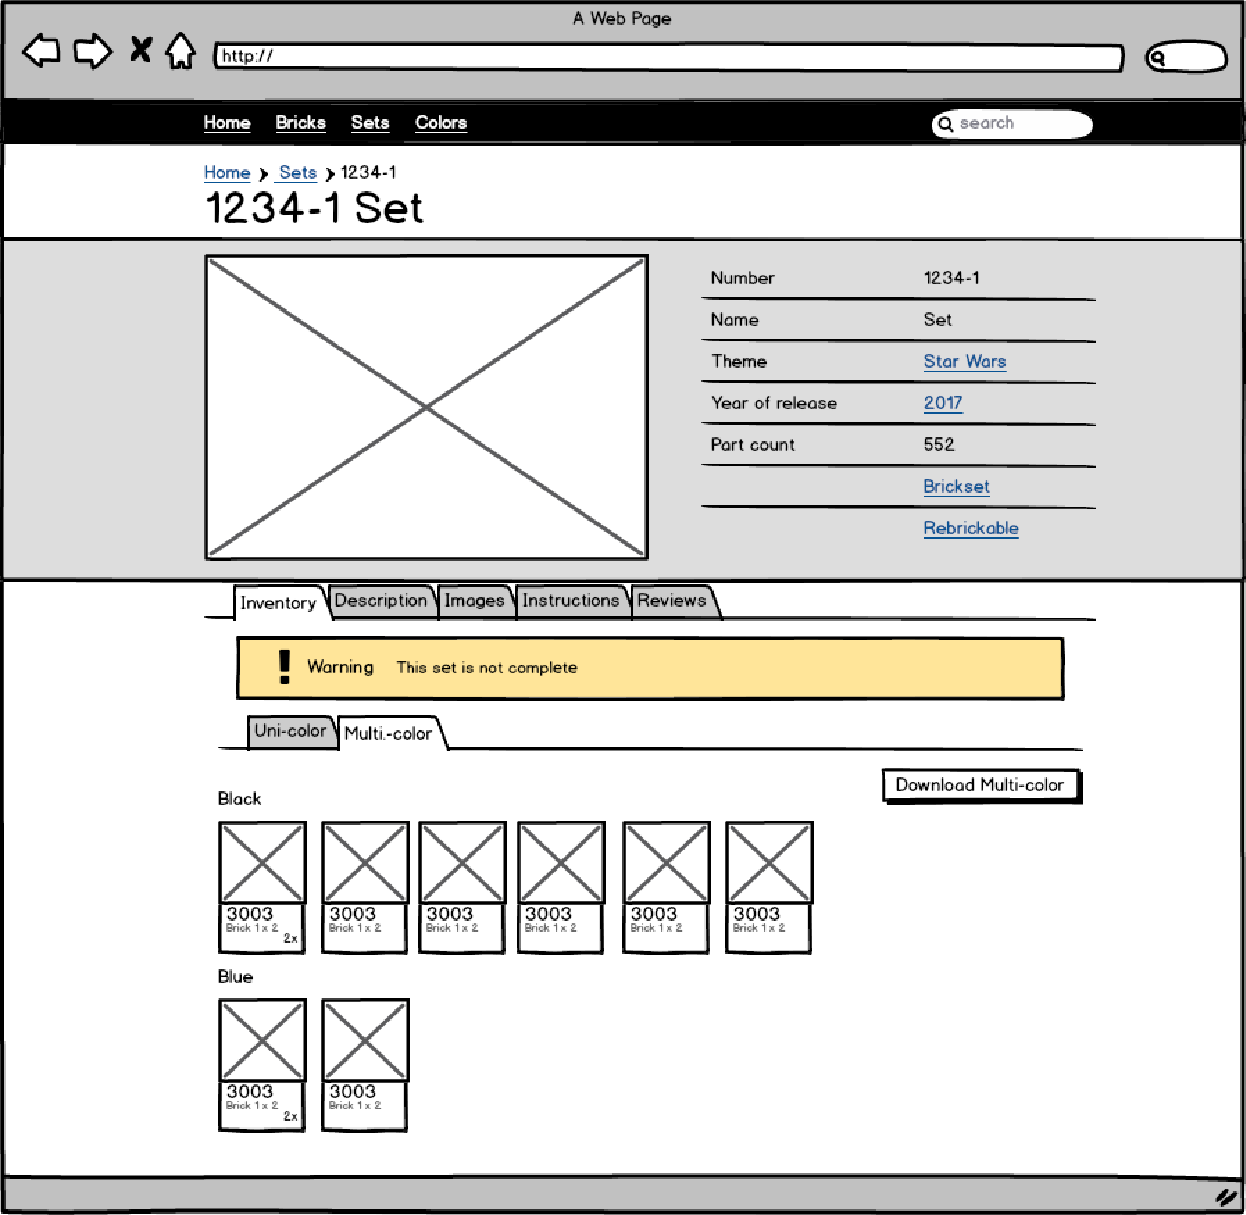
\includegraphics[width=\textwidth,height=\textheight,keepaspectratio]{pdfs/wireframe_set.pdf}
    \caption{Návrh stránky detailu stavebnice}\label{wireframe-stavebnice-detail}
\end{figure}

\subsection{Detail součástky}
Stránka detailu součástky (obrázek \emph{\ref{wireframe-soucastka-detail}}) je navržena podobně jako stránka detailu stavebnice. 

Hlavní blok obsahuje obrázek součástky a přehled atributů. Obrázek součástky má v~pravém horním rohu tlačítko, kterým se spouští interaktivní 3D náhled. Dále blok obsahuje tlačítko pro stažení 3D modelu. 

Druhý blok obsahuje dvě podstránky. První podstránka zobrazuje všechny příbuzné součástky. V~druhé je možné prohlížet veškeré stavebnice, ve kterých se součástka vyskytuje.

\begin{figure}[htbp]
    \centering
    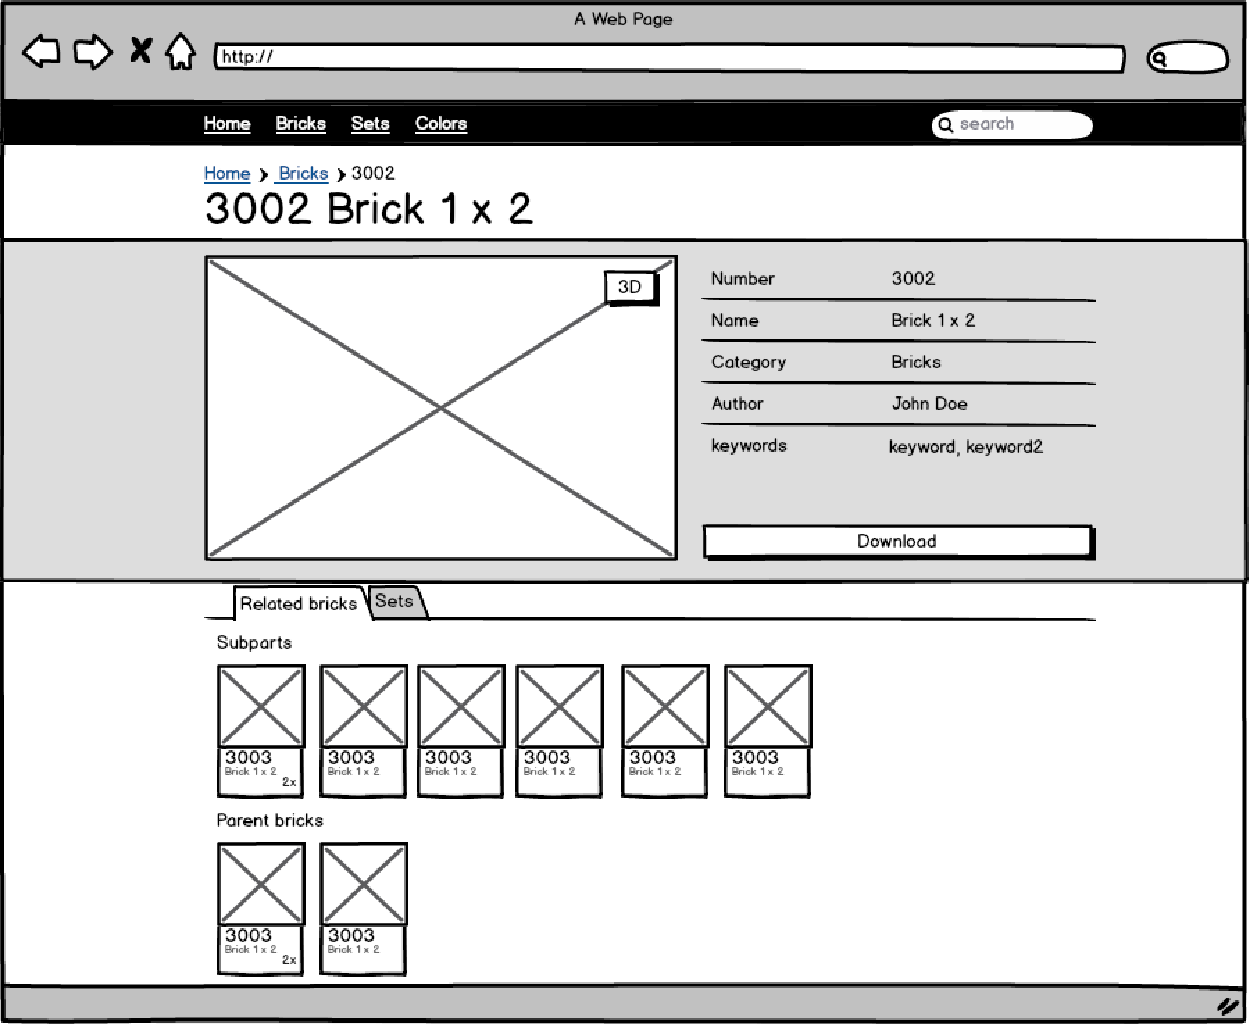
\includegraphics[width=\textwidth,height=\textheight,keepaspectratio]{pdfs/wireframe_brick.pdf}
    \caption{Návrh stránky detailu součástky}\label{wireframe-soucastka-detail}
\end{figure}

\subsection{Seznam barev}
Stránka seznamu barev (obrázek \emph{\ref{wireframe-barvy}}) slouží uživatelům k~seznámení se s~možnými barevnými variantami součástek. Barvy jsou zobrazeny ve dvou tabulkách. První tabulka sdružuje klasické barvy a druhá transparentní barvy. 

Tato stránka podle původního návrhu sloužila k možnosti dohledání přesné barvy součástky podle jména barvy. Později byla však tato informace zahrnuta přímo na místa, kde se vyskytuje zmínka o barvě. Tato stránka tedy postrádá svůj původní význam a mohla by být odstraněna.

\begin{figure}[htbp]
    \centering
    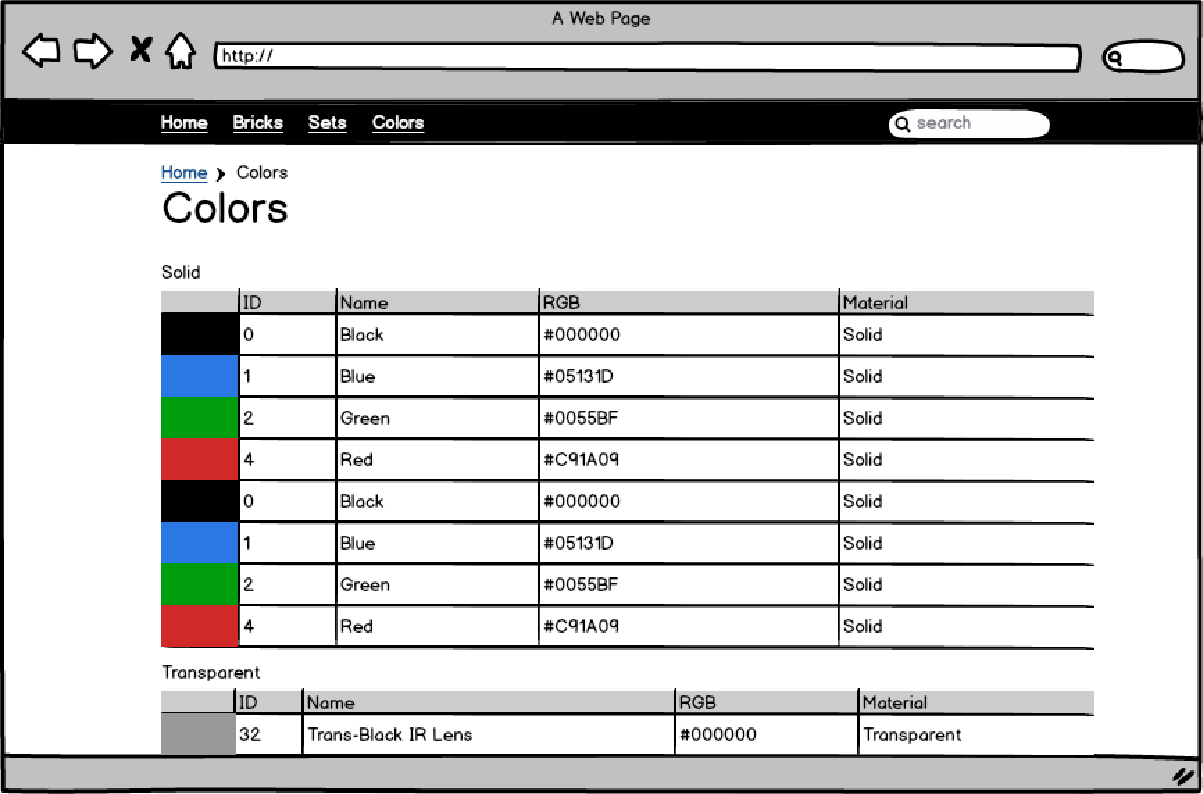
\includegraphics[width=\textwidth,height=\textheight,keepaspectratio]{pdfs/wireframe_colors.pdf}
    \caption{Návrh stránky seznamu barev}\label{wireframe-barvy}
\end{figure}
\chapter{Implementace} 
\section{Použité technologie}\label{implementace-technologie}

\subsection{Framework Symfony}  
Symfony je sada znovupoužitelných komponent PHP a PHP framework pro tvorbu webových projektů \autocite{symfony}. Jedná se o~jeden z~celosvětově nejpoužívanějších nástrojů pro tvorbu webových stránek \autocite{php-frameworky}.

\subsection{Komponenty}
Při implementaci aplikace byla kromě základních komponent frameworku Symfony využita celá řada dalších komponent třetích stran:

    \paragraph{KnpMenuBundle}
    integruje do Symfony PHP knihovnu KnpMenu, která usnadňuje vytváření navigací v~aplikaci. \autocite{knpmenu} 

    \paragraph{KnpPaginatorBundle}
    integruje do Symfony PHP knihovnu KnpPagerComponent, která usnadňuje stránkování kolekcí. \autocite{knppaginator}
    
    \paragraph{LiipImagineBundle}
    poskytuje nástroj pro manipulaci s~obrázky. Umožňuje vytváření miniatur, změnu velikosti obrátku a další transformace. \autocite{liipimagine}

    \paragraph{OneupFlysystemBundle}
    je abstrakce souborového systému, která umožňuje snadnou práci se soubory a jednoduchou výměnu lokálního souborového systému za vzdálený. \autocite{oneupflysytem}
   
    \paragraph{FOSElasticaBundle}
    poskytuje integraci knihovny Elastica \autocite{elastica}, zajišťující komunikaci s~vyhledávačem Elasticsearch \autocite{elasticsearch} do Symfony. \autocite{foselastica}  
   
    \paragraph{DoctrineCacheBundle} 
    umožňuje využívání různých cachovacích systémů poskytovaných knihovnou Doctrine Cache. \autocite{doctrinecache}

\subsection{Databáze}
Framework Symfony používá pro persistenci dat \gls{ORM} Doctrine 2. Dotazy na databázi se provádějí přes entity manager a třídy
repozitářů (ve kterých jsou definované složitější dotazy), které entity manager využívají. V~Doctrine 2 mají třídy anotované atributy, které se mají persistovat. Pomocí anotací jsou definované vztahy mezi třídami, datové typy sloupců databáze a mapování.

Pro vývoj a běh aplikace jsem použil MySQL, který je druhým nepoužívanějším databázovým serverem \autocite{database-servers}. Zároveň by však vzhledem k~abstrakci poskytované knihovou Doctrine 2 bylo možné zvolit i jiný databázový server (s~nutností zohlednění při implementaci načítání CSV tabulek Rebrickable, popsané v~sekci \ref{nacitani-rebrickable}).

\subsection{Front-end}
Pro usnadnění práce při tvorbě projektu poskytujícího uživatelské rozhraní je vhodné využítí front-end framoworku. Frameworky definují vzhled a chování nejzákladnějších, často používaných prvků. 

Pro tvorbu práce jsem se rozhodoval kromě využití pro mě již známého framworku Bootstrap 3 také nad možností využití dalších nejpoužívanějších alternativ – Foundation a Sematnic UI \autocite{web:frameworks}. Pro mou aplikaci jsem se nakonec rozhodnul využít frameworku Semantic UI. Semantic UI při definování tříd používá přirozené názvy vycházející z~angličtiny, tudíž je jeho použití velmi intuitivní a naučení používání by mělo být velmi snadné. V~ukázce kódu \ref{ukazka-semantic} je možné vidět příklad definice mřížky se třemi sloupečky pomocí Sematnic UI.

\begin{listing}[htbp]
  \begin{minted}{html}
<div class="ui three column grid">
  <div class="row">
    <div class="column"></div>
    <div class="column"></div>
    <div class="column"></div>
  </div>
</div>
    \end{minted}
  \caption{Ukázka definice mřížky pomocí Semantic UI\label{ukazka-semantic}}
\end{listing}

\section{Architektura}
Architektura aplikace je členěna do tří balíků reprezentující logicky odlišné funkční celky. Hierarchie balíků je znázorněna na diagramu \ref{diagram-bundles}.

\begin{figure}[htbp]
    \centering
    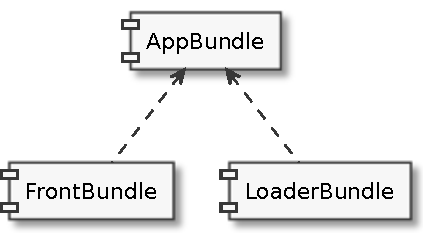
\includegraphics[width=0.5\textwidth,height=\textheight,keepaspectratio]{pdfs/bundles}
    \caption{Architektura komponent\label{diagram-bundles}}
\end{figure}

\paragraph{AppBundle}  
je základním balíkem aplikace obsahující implementaci datové vrstvy aplikace, zodpovědné za persistenci dat a jejich zpřístupnění. Dále obsahuje implementaci klienta pro přístup k datům Brickset přes API a implementaci business logiky aplikace.

\paragraph{FrontBundle} 
obsahuje implementaci uživatelského rozhraní aplikace v podobě \textit{Controller} tříd a \textit{Twig} šablon sloužících k zobrazení dat uživateli.

\paragraph{LoaderBundle} 
zastřešuje logiku aplikace pro načítání součástek knihovny LDraw a databáze Rebrickable z \gls{CSV} souborů za pomoci konzolových příkazů \autocite{symfony:console}. 



\section{Načítání dat}

\subsection{Načítání knihovny LDraw}
Mechanizmus načítání a aktualizace knihovny LDraw je implementován s~využitím Symfony komponenty Console. Administrátor aplikace může spouštět jednotilvé příkazy podle instrukcí uvedených v~dodatku \ref{append:instalace}. Na základě těchto příkazů jsou následně načítána data do databáze a prováděn převod formátu. V~ukázce kódu \ref{ukazka-prikaz-ldraw} je možné vidět volání příkazu pro načtení knihovny LDraw.

\begin{listing}[htbp]
        \begin{minted}{bash}
$ bin/console app:load:ldraw --all
------------------------------------------------------------------------
Downloading LDraw library
------------------------------------------------------------------------
Loading file from: http://www.ldraw.org/library/updates/complete.zip
[33.93 MB / 33.93 MB] [===========================]  100% (1 min/1 min)
LDraw libary downloaded
------------------------------------------------------------------------
Loading models from LDraw library: /tmp/printabrick.HIH6lN/ldraw/
------------------------------------------------------------------------
[9782 / 9782] [===========================] 100% (6 mins/6 mins) 
Done with "0" errors.
        \end{minted}
    \caption{Ukázka příkazu pro načtení knihovny LDraw\label{ukazka-prikaz-ldraw}}
\end{listing}

Aplikace umožňuje načítání a aktualizaci celé knihoviny i jednotlivých součástek. Proces načítání jednotlivé součástky je znázorněn na diagramu \ref{schema-nacitani} a podrobněji popsán v~následujících podsekcích.

\begin{figure}[htbp]
    \centering
    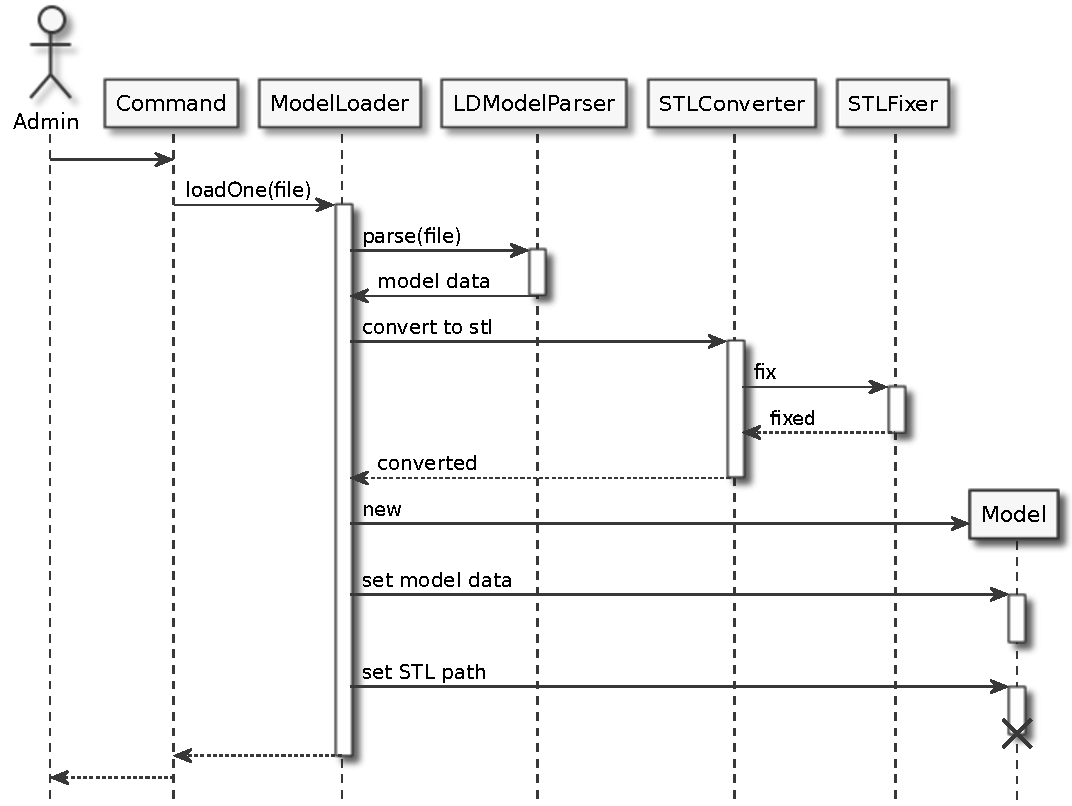
\includegraphics[width=\textwidth,height=\textheight,keepaspectratio]{pdfs/loading.pdf}
    \caption{Diagram načítání součástky knihovny LDraw \label{schema-nacitani}}
\end{figure}

\subsubsection*{Parsování součástek LDraw}
Parsování součástek formátu LDraw má na starost třída \textit{LDModelParser}. Třída na základě specifikace formátu LDraw představeného v~sekci \ref{ldraw-format} parsuje hlavičku souboru i reference na podsoučástky. Data jsou následně v~podobě asociativního pole vrácena k~dalšímu zpracování.

\subsubsection*{Převod formátu}
Pro spouštění programů zajišťujících převod formátu LDraw na formát \textit{\gls{STL}} jsem využil komponenty Symfony Process \autocite{symfony:process}. Ta umožňuje spouštění příkazů přímo z~kódu PHP (ukázka kódu \ref{ukazka-stlconverter}).

Převod formátu je nejprve zajištěn třídou \textit{STLConverter}, která zastřešuje volání programu LDView (představeného v~sekci \ref{podsekce-ldview}). Následně třída \textit{STLFixer} provede opravu \textit{\gls{STL}} souboru pomocí volání programu ADMesh (představeného v~sekci \ref{podsekce-admesh}).


\begin{listing}[htbp]
        \begin{minted}{php}
/**
 * Call LDView process with $arguments.
 *
 * @param array $arguments
 */
private function runLDView(array $arguments)
{
    $builder = new ProcessBuilder();
    $process = $builder
        ->setPrefix($this->ldview)
        ->setArguments($arguments)
        ->getProcess();

    $process->run();

    if (!$process->isSuccessful()) {
        throw new ProcessFailedException($process);
    }
}
        \end{minted}
    \caption{Ukázka použití komponenty Symfony Process \label{ukazka-stlconverter}}
\end{listing}

\subsubsection*{Logování}
Protože během procesu načítání knihovny dochází ke zpracování velkého množství dat a ne vždy se dá spoléhat na validitu vstupu, bylo třeba implementovat mechanizmus logování událostí. Významné události a chyby jsou logovány pomocí knihovny Monolog \autocite{symfony:monolog}. Ukázku přidávání události do logu je možné vidět v~ukázce kódu \ref{ukazka-log-udalost} a podobu souboru logu v~ukázce kódu \ref{ukazka-log}.

\begin{listing}[htbp]
        \begin{minted}{php}
try {
    $modelArray = $this->ldModelParser->parse(file_get_contents($file));
} catch (ParseErrorException $e) {
    $this->logger->error($e->getMessage(), [$file]);

    return null;
} catch (FileException $e) {
    $this->logger->error($e->getMessage(), [$file]);

    return null;
}
        \end{minted}
    \caption{Ukázka použití knihovny Monolog \label{ukazka-log-udalost}}
\end{listing}

\begin{listing}[htbp]
        \begin{minted}{text}
[2017-05-27 22:54:05] loader.INFO: Model skipped. {"number":"004695a","type":"Sticker"} []
[2017-05-27 22:54:05] loader.INFO: Model skipped. {"number":"004695b","type":"Sticker"} []
[2017-05-27 22:54:05] event.ERROR: Subpart file not found {"subpart":"2-4cyli","model":"3820"} []
        \end{minted}
    \caption{Ukázka logu načítání\label{ukazka-log}}
\end{listing}

\subsection{Načítání dat Rebrickable}\label{nacitani-rebrickable}
Načítání velkého množství dat z~CSV souborů do aplikace může být dle \autocite{grok} velmi problematické. Načítání databáze Rebrickable má na starost služba \textit{RebrickableLoader}. Ta pomocí volání MySQL funkce \mintinline{text}{LOAD DATA LOCAL INFILE} (viz ukázka kódu \ref{ukazka-nacitani-csv}) načítá velmi rychle CSV soubory Rebrickable.

\begin{listing}[htbp]
        \begin{minted}{php}
private function loadCsvFile($file, $table, $columns)
{
    $query = sprintf("LOAD DATA LOCAL INFILE '%s' 
        REPLACE INTO TABLE %s
        CHARACTER SET UTF8
        FIELDS TERMINATED BY ',' OPTIONALLY ENCLOSED BY '\"'
        LINES TERMINATED BY '\\n'
        IGNORE 1 LINES %s", addslashes($file), $table, $columns);

    return $this->em->getConnection()->prepare($query)->execute();
}
        \end{minted}
    \caption{Ukázka načítání tabulek CSV \label{ukazka-nacitani-csv}}
\end{listing}

\subsection{Mapování LDraw a Rebrickable}
Jedním z~problémů, který vyvstává při využití různých zdrojů dat pro obdržení 3D modelů součástek a databáze stavebnic, je vzájemné provázání těchto dat. Namapování součástek má na starost třída \textit{RelationMapper}, která provádí přiřazení součástek z~knihovny LDraw k~součástkám z~databáze Rebrickable. 

Protože obě služby používají lehce odlišný systém číslování součástek (i přes fakt, že číslování Rebrickable vychází z~LDraw), nelze při zohlednění všech pravidel LDraw \autocite{ldraw:numbering:faq} i Rebrickable \autocite{rebrickable:numbering:changes} automaticky rozpoznat vazby všech součástek.

K~umožnění manuálního přiřazení součástek LDraw k spoučástkám Rebrickable jsem implementoval mechanizmus umožňující definování vazeb pomocí \gls{YAML} souboru \textit{app/Resources/relations/part\_model.yml}. K~načtení souboru je využita komponenta Symfony Yaml Component \autocite{symfony:yaml}. Ukázku mapování součástky na model je možné vidět v~ukázce kódu \ref{ukazka-parovani}. Tyto vazby jsou následně zohledněny při běhu příkazu pro spárování součástek.

\begin{listing}[htbp]
        \begin{minted} {yaml}
#rebrickable_part_ID: ldraw_model_ID
970d00: 970c00
298c04: 4592c01
        \end{minted}
    \caption{Ukázka part\_model.yml \label{ukazka-parovani}}
\end{listing}

\subsection{API Brickset}
Dalším zdrojem dat využívaným pro obdržení informací o~stavebnicích je API Brickset. Jak již bylo zmíněno v~sekci \ref{reserse-brickset}, API Bricsket je implementováno jako služba postavená nad protokolem \gls{SOAP}. V~PHP je pro komunikaci se SOAP servery k~dispozici třída \textit{SOAPClient} \autocite{soapclient}, která za nás obstarává komunikaci na základě definice v~podobě \gls{WSDL} souboru. 

Při získávání statických dat přes API je vhodné využít možnosti cachování k~minimalizaci počtu dotazů na server a k~urychlení načítání dat. K~tomuto jsem využil komponenty DoctrineCacheBundle. V~ukázce kódu \ref{ukazka-cache} je zobrazena metoda \mintinline{php}{getSetInstructions} třídy \textit{BricksetManager}, která načítá insturkce k~postavení stavebnice z~cache (pokud se zde data již vyskytují) nebo pomocí Brickset API. 

\begin{listing}[htbp]
        \begin{minted} {php}
public function getSetInstructions($id)
{
    $key = 'instructions-'.$id;

    if (!$data = unserialize($this->cache->fetch($key))) {
        $data = $this->bricksetClient->getInstructions($id);
        $this->cache->save($key, serialize($data), self::CACHE_LIFETIME);
    }

    return $data;
}
        \end{minted}
    \caption{Ukázka načtení instrukcí stavebnice\label{ukazka-cache}}
\end{listing}


\section{3D náhled}
3D náhled součástek LEGO je implementován s využitím JavaScriptového frameworku Three.js. Tento frameworku disponuje velmi rozsáhlou a přehlednou dokumentací, včetně ukázek použití a je nejpoužívanějsím JavaScriptovým WebGL frameworkem \autocite{webgl-comparison}. Na základě těchto důvodů bylo rozhodnuto o jeho využití v tomto projektu.

% Three.js
% OrbitControls.js
% STLLoader.js

% \begin{listing}[htbp]
%         \begin{minted}{javascript}
%  $('#model-viewer').ModelViewer('{{ path('media_file', {'path':model.path}) }}');
%   \end{minted}
%   \caption{Inicializace 3D náhledu\label{modelviewer-initialization}}
% \end{listing}

% \begin{listing}[htbp]
%     \begin{minted}{javascript}
% ModelViewer.prototype.loadStl = function(model) {
%     var self = this;
%     var loader = new THREE.STLLoader();

%     loader.load(model,
%         function (geometry) {
%             self.addModel(geometry);
%         },
%         function(progress) {},
%         // Show error message
%         function(error) {
%             self.showError();
%         }
%     );
% };
%     \end{minted}
%     \caption{Načtení STL modelu pomocí Three.js\label{modelviewer-stl}}
% \end{listing}

Na obrázku \ref{obrazek-ldraw-shortcut} je možné vidět ukázku a možnosti implementovaného 3D náhledu.

\begin{figure}[htbp]
        \centering
        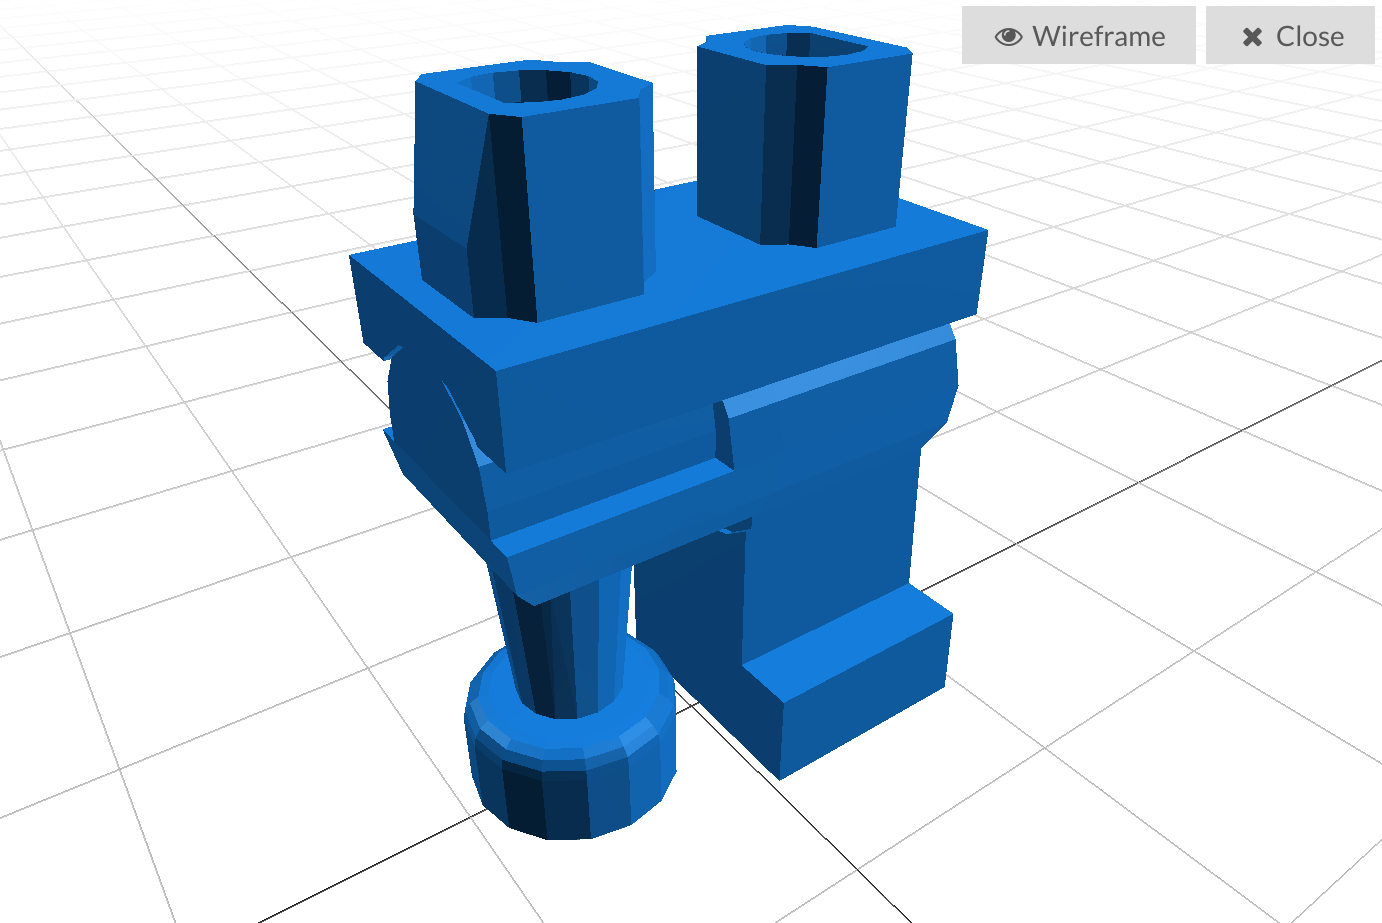
\includegraphics[width=0.48\textwidth,height=\textheight,keepaspectratio]{images/model-viewer-solid.png}
        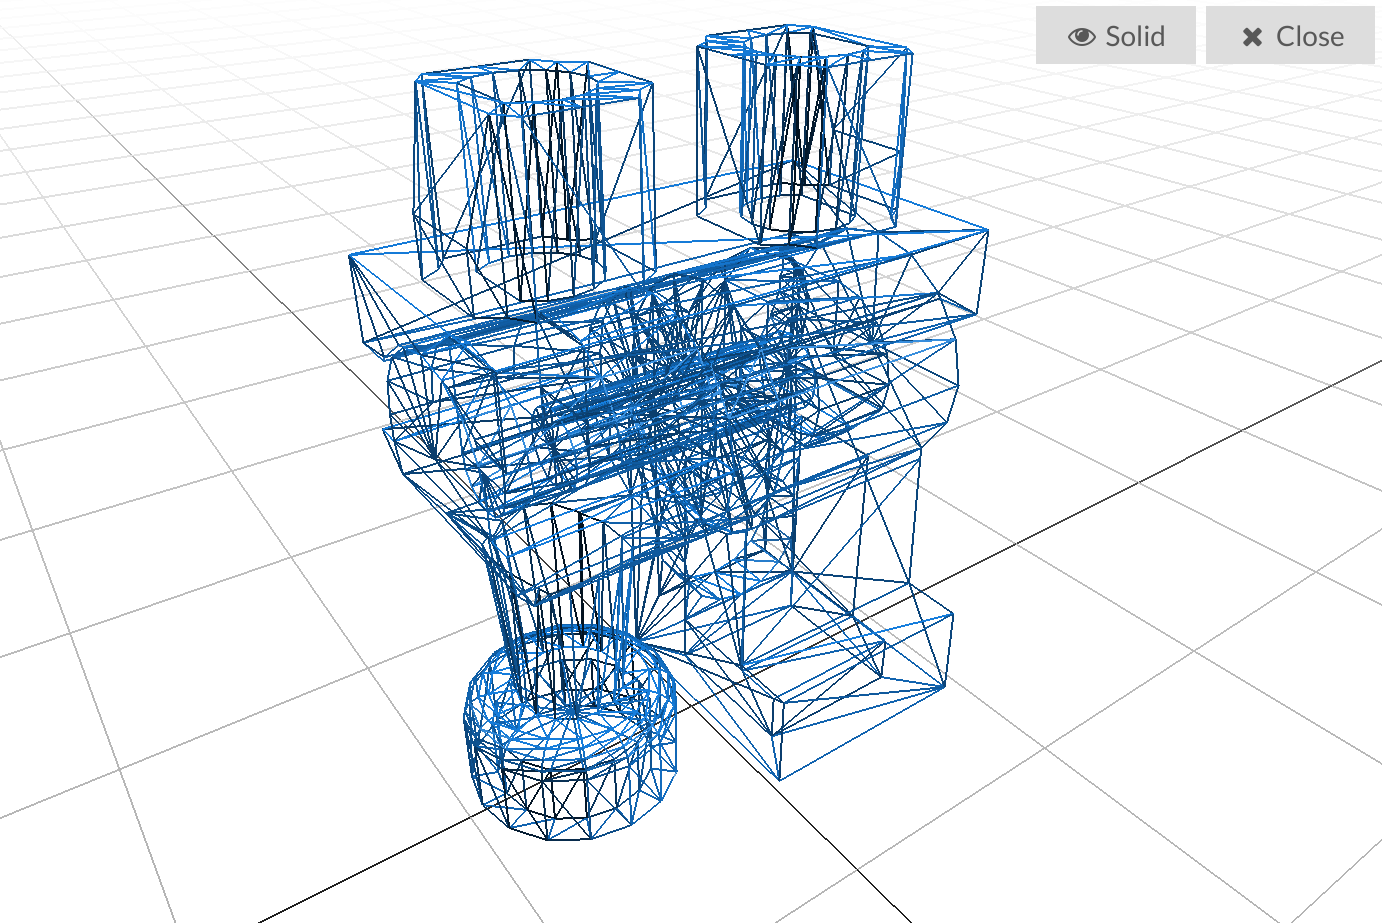
\includegraphics[width=0.48\textwidth,height=\textheight,keepaspectratio]{images/model-viewer-wireframe.png}
        \caption{3D náhled součástky \label{obrazek-ldraw-shortcut}}
\end{figure}

\section{Stažení součástek}
Poskytnutí ZIP archivů s~modely součástek má na starost služba \textit{ZipService}. Ta s~využitím knihovní třidy PHP \textit{ZIPArchive} umožňuje vytvoření archivů, které jsou následně poskytnuté uživateli ke stažení. 

V~ukázce adresářové struktury \ref{ldraw-archiv} je možné vidět strukturu archivu stavebnice roztříděné podle barev.

\begin{dirfigure}%
    \dirtree{%
        .1 2000416-1\_Duck(Multi-Color).
            .2 Red\_(\#C91A09)\DTcomment{složka se součástkami v~červené barvě}.
                .3 3021\_(2x).stl.
            .2 Yellow\_(\#F2CD37)\DTcomment{složka se součástkami ve žluté barvě}.
                .3 3001\_(1x).stl.
                .3 3003\_(2x).stl.
                .3 3004\_(1x).stl.    
            .2 LICENSE.txt \DTcomment{licenční ujednání se seznamem autorů součástek}.
    }
    \caption{Obsah archivu 2000416-1\_Duck(Multi-Color).zip}\label{ldraw-archiv}
\end{dirfigure}

\section{Obrázky součástek a stavebnic}
\subsection{Renderování součástek}
Jak již bylo zmíněno v~sekci \emph{\ref{reserse-vykresleni}}, Rebrickable poskytuje většinu obrázků vyrenderovaných součástek z~knihovny LDraw volně ke stažení. Pro zbytek součástek jsem implementoval mechanizmus vykreslení s~využitím programů stl2pov \autocite{stl2pov} a POV-ray \autocite{povray}.

Vykreslení součástek zajišťuje třída \textit{STLRenderer}. Třída nejprve připraví kompletní scénu, obsahující součástku převedenou pomocí stl2pov do POV-ray formátu. Dále scéna obsahuje definici pozice světel a kamery, specifikované v~souboru \textit{app/Resources/povray\_layout/layout.tmpl}. Následně je pomocí volání programu POV-ray vykreslen obrázek. 

Porovnání vyrenderované součástky s~obrázkem součástky z~Rebrickable je možné vidět na obrázku \emph{\ref{porovnani-render}}.

\begin{figure}[htbp]
    \centering
    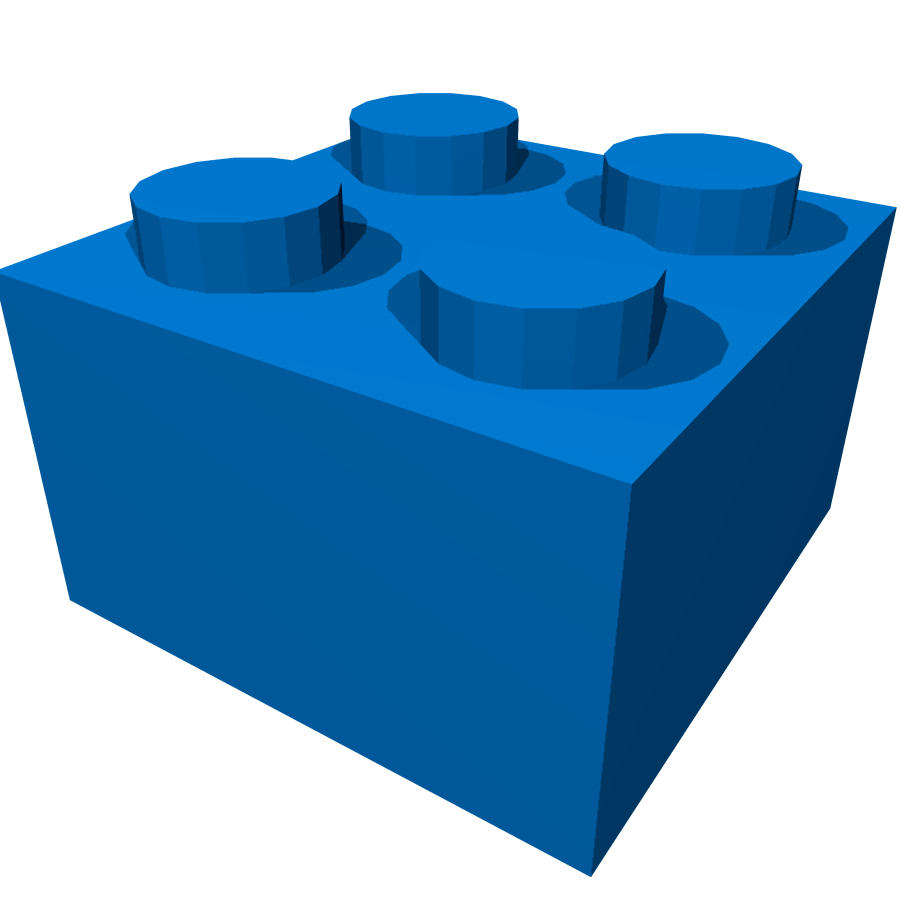
\includegraphics[width=0.30\textwidth,height=\textheight,keepaspectratio]{images/povray.png}
    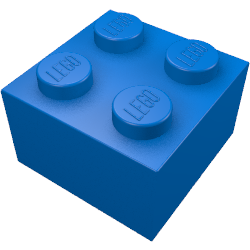
\includegraphics[width=0.30\textwidth,height=\textheight,keepaspectratio]{images/3003.png}
    \caption{Porovnání renderu součástky a Rebrickable \autocite{rebrickable:part:image:3003}\label{porovnani-render}}
\end{figure}


\subsection{Cachování obrázků}
Pro urychlení načítaní webových stránek jsem implementoval mechanizmus cachování miniatur obrázků součástek a stavebnic. K~práci s~obrázky v~Symfony slouží komponenta LiipImagineBundle \autocite{liipimagine}. LiipImagineBundle umožňuje definování různých filtrů a transformací, které jsou aplikovány na zobrazované obrázky. Transformované obrázky jsou následně uloženy do cache, ze které jsou při dalším požadavku načtené.

Proces vytváření transformovaných obrázků se zakládá ze tří kroků:
\begin{enumerate}
    \item načtení obrázku,
    \item aplikace flitrů,
    \item uložení transformovaného obrázku do cache.
\end{enumerate}

\subsubsection*{Načtení obrázku}
Načítání obrázků mají na starosti třídy \textit{PartImageLoader} a \textit{SetImageLoader}, které implementují rozhraní \textit{LoaderInterface} a na základě vstupu vrací binární obsah obrázku. 

% \subsubsection*{PartImageLoader}
% Třída \textit{PartImageLoader} má na starost vyhledávání obrázku součástek na základě zadané cesty. 


% \subsubsection*{SetImageLoader}


% http://rebrickable.com/media/parts/ldraw/1/3003.png

\subsubsection*{Aplikace filtrů}
Filtry jsou na obrázky aplikovány na základě konfigurace (ukázka kódu \emph{\ref{liip-imagine-config}}).  

\begin{listing}[htbp]
  \begin{minted}{yaml}
liip_imagine:
    filter_sets:
        part_min:
            quality: 90
            data_loader: part_image_loader
            cache: ~
            default_image: "/resources/images/noimage_min.png"
            filters:
                upscale: { min: [230, 230] }
                thumbnail: { size: [230, 230], mode: inset, allow_upscale: true }
                background: { size: [250, 250], position: center, color: '#FFFFFF' }
  \end{minted}
  \caption{Ukázka konfigurace filtru LiipImagineBundle\label{liip-imagine-config}}
\end{listing}



% \begin{listing}[htbp]
%   \begin{minted}{html}
% <img src="{{ 1/3003.png | imagine_filter(part_min) }}" >
%     \end{minted}
%   \caption{Ukázka použití filtru LiipImagineBundle\label{liip-imagine-usage}}
% \end{listing}   


\section{Vyhledávání}
Podle funkčního požadavku \ref{fp:model:search} musí aplikace umožňovat vyhledávání a procházení součástek a stavebnic. Jak již bylo zmíněno v~podkapitole \ref{implementace-technologie}, k~realizaci tohoto požadavku jsem využil fulltextového vyhledávače Elasticsearch \autocite{elasticsearch}. Pro implemetaci konkrétně balíček FOSElasticaBundle \autocite{foselastica}, který integruje PHP knihovu pro komunikaci s~Elasticsearch serverem přes \gls{REST} API do frameworku Symfony.

% \subsection{Konfigurace}
% \begin{listing}[htbp]
%   \begin{minted}{yaml}
% fos_elastica:
%   clients:
%     default: { host: '%elastica_host%', port: '%elastica_port%' }
%   indexes:
%     app:
%       index_name: app_%kernel.environment%
%       settings:
%         index:
%           analysis:
%             analyzer:
%               name_analyzer:
%                 type:       custom
%                 tokenizer:  nGram
%                 filter:     [lowercase,stopwords]
%               id_analyzer:
%                 type:       custom
%                 tokenizer:  edge_ngram
%             tokenizer:
%               nGram:
%                 type:       nGram
%                 min_gram:   3
%                 max_gram:   20
%               ...
%             filter:
%               ...
%   \end{minted}
%   \caption{Ukázka konfigurace Elasticsearch\label{elasticsearch-config}}
% \end{listing}

\subsection{Nastavení indexování}
Vyhledávání a filtrování kolekce probíhá na základě nastavených pravidel indexování enitit. Ukázku nastavení indexování entity \textit{Set} je 
možné vidět v~ukázce kódu \ref{elasticsearch-set-index}. Nastavní probíhá pomocí konfiguračního souboru ve formátu \gls{YAML} a určuje atributy společně s~metodou indexace.

\begin{listing}[htbp]
  \begin{minted}{yaml}
fos_elastica:
  indexes:
    app:
      types:
        set:
          mappings:
            id:
              type: "keyword"
              fields:
                ngrams: { type: 'text', analyzer: id_analyzer }
            name: 
              analyzer: name_analyzer 
              search_analyzer: "standard"
            year: { type: integer }
            partCount: { type: integer }
            theme:
              type: "object"
              properties: { id: ~ }
          persistence:
            driver: orm
            model: AppBundle\Entity\Rebrickable\Set
            ...
            repository: AppBundle\Repository\Search\SetRepository
            ...
  \end{minted}
  \caption{Ukázka nastavení mapování entity \label{elasticsearch-set-index}}
\end{listing}

\subsection{Vyhledávání}
Vyhledávání je v~aplikaci zajišťováno službou \textit{SearchService}. Služba na základě formuláře s~využitím repozitářů připraví dotaz, který je následně odeslán na vyhledávací server Elasticsearch v~podobě zobrazené v~ukázce kódu \ref{elasticsearch-query}. Následně jsou získaná data z~odpovědi automaticky namapována na entity s~využitím Doctrine 2 a vrácen výsledek.

\begin{listing}[htbp]
  \begin{minted}{json}
{
  "query": {
    "bool": { 
      "must": [{
        "multi_match": {
          "fields": [ "name", "id", "id.ngrams" ],
          "query": "falcon", 
          "fuzziness": 0.7,
          "minimum_should_match": "80%",
          "operator": "and"
        }
      }],
      "filter": [
        { "match": { "theme.id" : 158 }},
        { "range": { "partCount" : { "gte" : "0", "lte" : "5922" }}},
        { "range": { "year" : { "gte" : "1950", "lte" : "2017" }}}
      ]
    }
  },
  "size": 500
}
        \end{minted}
  \caption{Ukázka JSON dotazu Elasticsearch\label{elasticsearch-query}}
\end{listing}

% \begin{listing}[htbp]
%   \begin{minted}{json}
% {
%     "took": 9, "timed_out": false, "_shards": { "total": 5, "successful": 5, "failed": 0 },
%     "hits": {
%         "total": 1, "max_score": 8.896875, 
%         "hits": [
%             {
%                 "_index": "app_dev", 
%                 "_type": "set",
%                 "_id": "75105-1",
%                 "_score": 8.896875,
%                 "_source": {
%                     "id": "75105-1",
%                     "name": "Millennium Falcon™",
%                     "year": 2015,
%                     "partCount": 1328,
%                     "theme": {
%                         "id": 158
%                     }
%                 }
%             }
%         ],
%     }
% }
%         \end{minted}
%   \caption{\label{elasticsearch-response}}
% \end{listing}


% \subsection{}

% \begin{listing}[htbp]
%   \begin{minted}{javascript}
% $('.ui.search')
%     .search({
%         type: 'category',
%         apiSettings: {
%             action: 'search',
%             url: routes.search_autocomplete+'?query={query}',
%         },
%         minCharacters: 3,
%         fields: {
%             title: 'name',
%             description: 'id',
%             url: 'url',
%             image: 'img'
%         }
%     });
%         \end{minted}
%   \caption{\label{semantic-search}}
% \end{listing}

% \section{Náhled pro sociální sítě}
Významným zdrojem návštěvnosti stránek mohou v~dnešní době být i sociální sítě. Aby byl sdílený odkaz na stránku dostatečně zajímavý je třeba stránky rozšířit o~patřičné meta informace. Facebook a většina sociálních sítí ke specifikování náhledu využívá protokol Open Graph představený firmou Facebook v~roce 2010 \autocite{opengraph}.

\begin{listing}[htbp]
  \begin{minted}{twig}

    <meta property="og:title" content="{{ title }}">
    <meta property="og:description" content="{{ description }}">
    <meta property="og:url" content="{{ url }}">
    <meta property="og:image" content="{{ image }}">
    <meta property="og:image:width" content="{{ imageWidth }}">
    <meta property="og:image:height" content="{{ imageHeight }}">
    <meta property="og:site_name" content="{{ name }}">

    <meta property="twitter:card" content="summary">

  \end{minted}
  \caption{\label{opengraph-meta}}
\end{listing}

\begin{figure}[htbp]
        \centering
        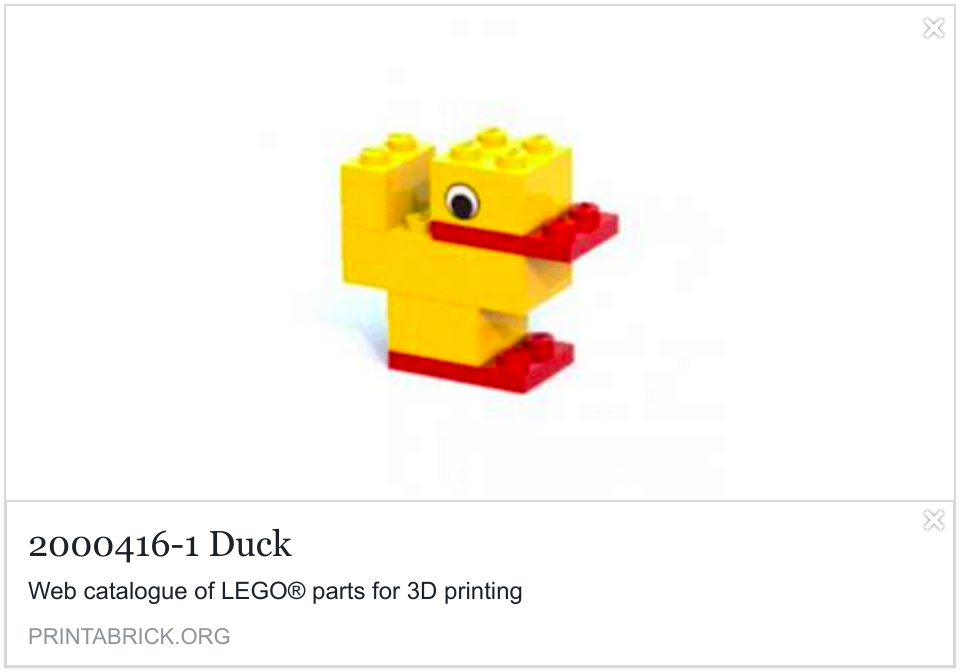
\includegraphics[width=\textwidth,height=\textheight,keepaspectratio]{images/fbshare.png}
        \caption{\label{facebook-share}}
\end{figure}

\chapter{Testování a nasazení}

\section{Testování}
V této sekci jsou popsány způsoby, jakými byla aplikace testována. K testování bylo využito jak metodik statické analýzy kvality kódu, tak i automatické testování pomocí jednotkových a integračních testů.

Statická analýza kvality kódu byla provedena nástrojem PHPSpec \autocite{phpspec}. Testování pomocí jednotkových a integračních testů bylo provedeno nástrojem PHPUnit \autocite{phpunit}.
Výstup testování pomocí PHPUnit se nachází v ukázce kódu \emph{\ref{phpunit-volani}}. 


\begin{listing}[htbp]
        \begin{minted}{console}
$ php vendor/bin/phpunit 
PHPUnit 6.2.2 by Sebastian Bergmann and contributors.

..................................................  50 / 121 ( 41%)
.................................................. 100 / 121 ( 82%)
.....................                              121 / 121 (100%)

Time: 41.4 seconds, Memory: 102.00MB

OK (121 tests, 191 assertions)
        \end{minted}
    \caption{Výstup PHPUnit testů \label{phpunit-volani}}
\end{listing}

 

 

\subsection{Pokrytí kódu testy}
Na obrázku \emph{\ref{phpunit-coverage}} je možné vidět pokrytí kódu testy, vygenerované pomocí PHPUnit.

\begin{figure}[htbp]
    \centering
    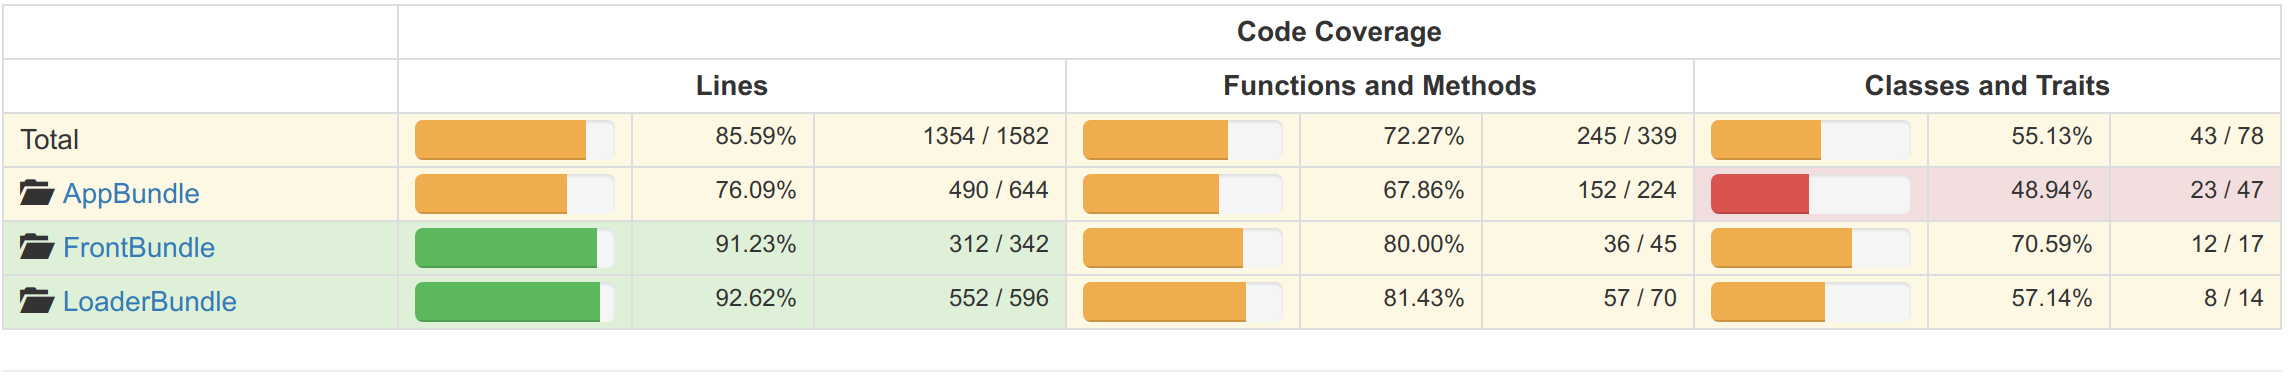
\includegraphics[width=\textwidth,height=\textheight,keepaspectratio]{images/coverage.png}
    \caption{Pokrytí kódu testy\label{phpunit-coverage}}
\end{figure}


\section{Nasazení}
Aplikace byla nasazena na školní \gls{VPS}, který byl speciálně zřízen pro potřeby mé aplikace. Na serveru běží operační systém CentOS 7 \autocite{centos}. Vzhedem k tomu, že jsem obdržel administrátorská práva k systému, bylo možné nainstalovat všechny potřebné závislosti, kterých aplikace využívá. 

Při instalaci bylo postupováno podle instalační příručky (příloha \emph{\ref{append:instalace}}), včetně úspešného běhu testů. 

Aplikace je nasazena a připravena k~používání na adrese \url{http://printabrick.org}. 



\chapter{Právní aspekty} 
V~této kapitole budou rozebrány právní aspekty výsledné aplikace, aby mohlo být rozhodnuto o~možnosti zveřejnění do sítě Internet. 

\section{Zdroje dat}
Při analyzování právních aspektů aplikace je v~první řadě nutné zhodnotit veškeré využité zdroje dat v~aplikaci. 

\subsection{LDraw}
Jak již bylo uvedeno v~sekci \emph{\ref{reserse-ldraw}}, všechny součástky knihovny LDraw jsou sdíleny pod licencí \gls{CC-BY} \autocite{CC-BY}.

Aby byla dodržena licence knihovny LDraw při sdílení 3D modelů součástek, je nutné spolu se staženými soubory jednoznačně uvést autora dle licence. Toho je docíleno přidáním souboru LICENSE.txt do sdíleného archivu. Příklad tohoto souboru je možné vidět v~ukázce kódu \emph{\ref{ukazka-licence}} zobrazující licenční soubor, zahrnutý v~archivu stavebnice \textit{2000416-1 Duck}. Dále je autor společně s licencí uveden na stránce detailu součástky.

\begin{listing}[htbp]
        \begin{minted}{text}
All stl files in this archive were converted by LDView from 
official LDraw Library http://www.ldraw.org/

Files are licensed under the Creative Commons - Attribution license.
http://creativecommons.org/licenses/by/2.0/

Attribution:

3021 - "Plate 2 x 3" by James Jessiman
3001 - "Brick 2 x 4" by James Jessiman
3003 - "Brick 2 x 2" by James Jessiman
3004 - "Brick 1 x 2" by James Jessiman
        \end{minted}
    \caption{Ukázka souboru LICENSE.txt\label{ukazka-licence}}
\end{listing}

\subsection{Rebrickable}
Jak již bylo řečeno v~kapitole \emph{\ref{reserse-rebrickable}}, Rebrickable poskytuje svá data volně bez nároků a omezení. Autoři Rebrickable pouze žádají o uvedení původu využívaných dat. Toto přání jsem splnil přidáním prohlášení do patičky každé stránky.

\subsection{Brickset}
API služby Brickset je volně dostupné k~vytváření doplňkových webových stránek nebo služeb bez uvedení omezujících podmínek. \autocite{brickset:key} 

\section{Obchodní značka LEGO}
Obchodní značka LEGO může být použita v~případě dodržení určitých podmínek i na neoficiálních webových stránkách, na kterých jsou zobrazovány nebo diskutovány prvky LEGO. Instrukce vydané společností LEGO jsou dostupné na \autocite{lego:fair-play}.

Shrnutí instrukcí: 
\begin{itemize}
        \item logo LEGO nesmí být použito na neoficiální webové stránce,
        \item obchodní značka LEGO by se měla při každém použití vždy zobrazovat se symbolem ®,
        \item musí být zřejmé, že stránka není sponzorována nebo autorizována společností LEGO,
        \item obchodní značka nesmí být zvýrazňována,
        \item značka LEGO nemůže být použita v~internetové adrese,
        \item stránka by měla obsahovat prohlášení o~popření právního nároku.
\end{itemize}

Všechny tyto instrukce byly zohledněny při tvorbě aplikace, včetně přidání prohlášení o~popření právního nároku do patičky (viz ukázka kódu \emph{\ref{ukazka-prohlaseni}}). Při tvorbě tohoto prohlášení jsem se inspiroval prohlášením z~patičky stránky služby Brickset \autocite{brickset:about}.

\begin{listing}[htbp]
        \begin{minted}{text}
LEGO®, the LEGO logo, the Minifigure, and the Brick and Knob 
configurations are trademarks of the LEGO Group of Companies which
does not sponsor, authorize, or endorse this site.
        \end{minted}
    \caption{Prohlášení o~popření právního nároku v~patičce stránky\label{ukazka-prohlaseni}}
\end{listing}

\section{Závěr}
Při implementaci byly zohledněny licenční podmínky všech služeb, využitých balíčků i instrukce společnosti LEGO pro neoficiální webové stránky a nebyly shledány žádné překážky k~zveřejnění. Výsledná webová aplikace tedy může být zveřejněna do sítě Internet.

\begin{conclusion}
  Cílem práce bylo navrhnout a implementovat webovou aplikaci umožňující stažení 3D modelů dílů LEGO. Tento cíl byl úspěšně naplněn včetně zveřejnění aplikace do sítě internet. 

Instance aplikace je nasazena a připravena k používání na adrese \url{http://printabrick.org}. 


\begin{figure}[htbp]
    \centering
    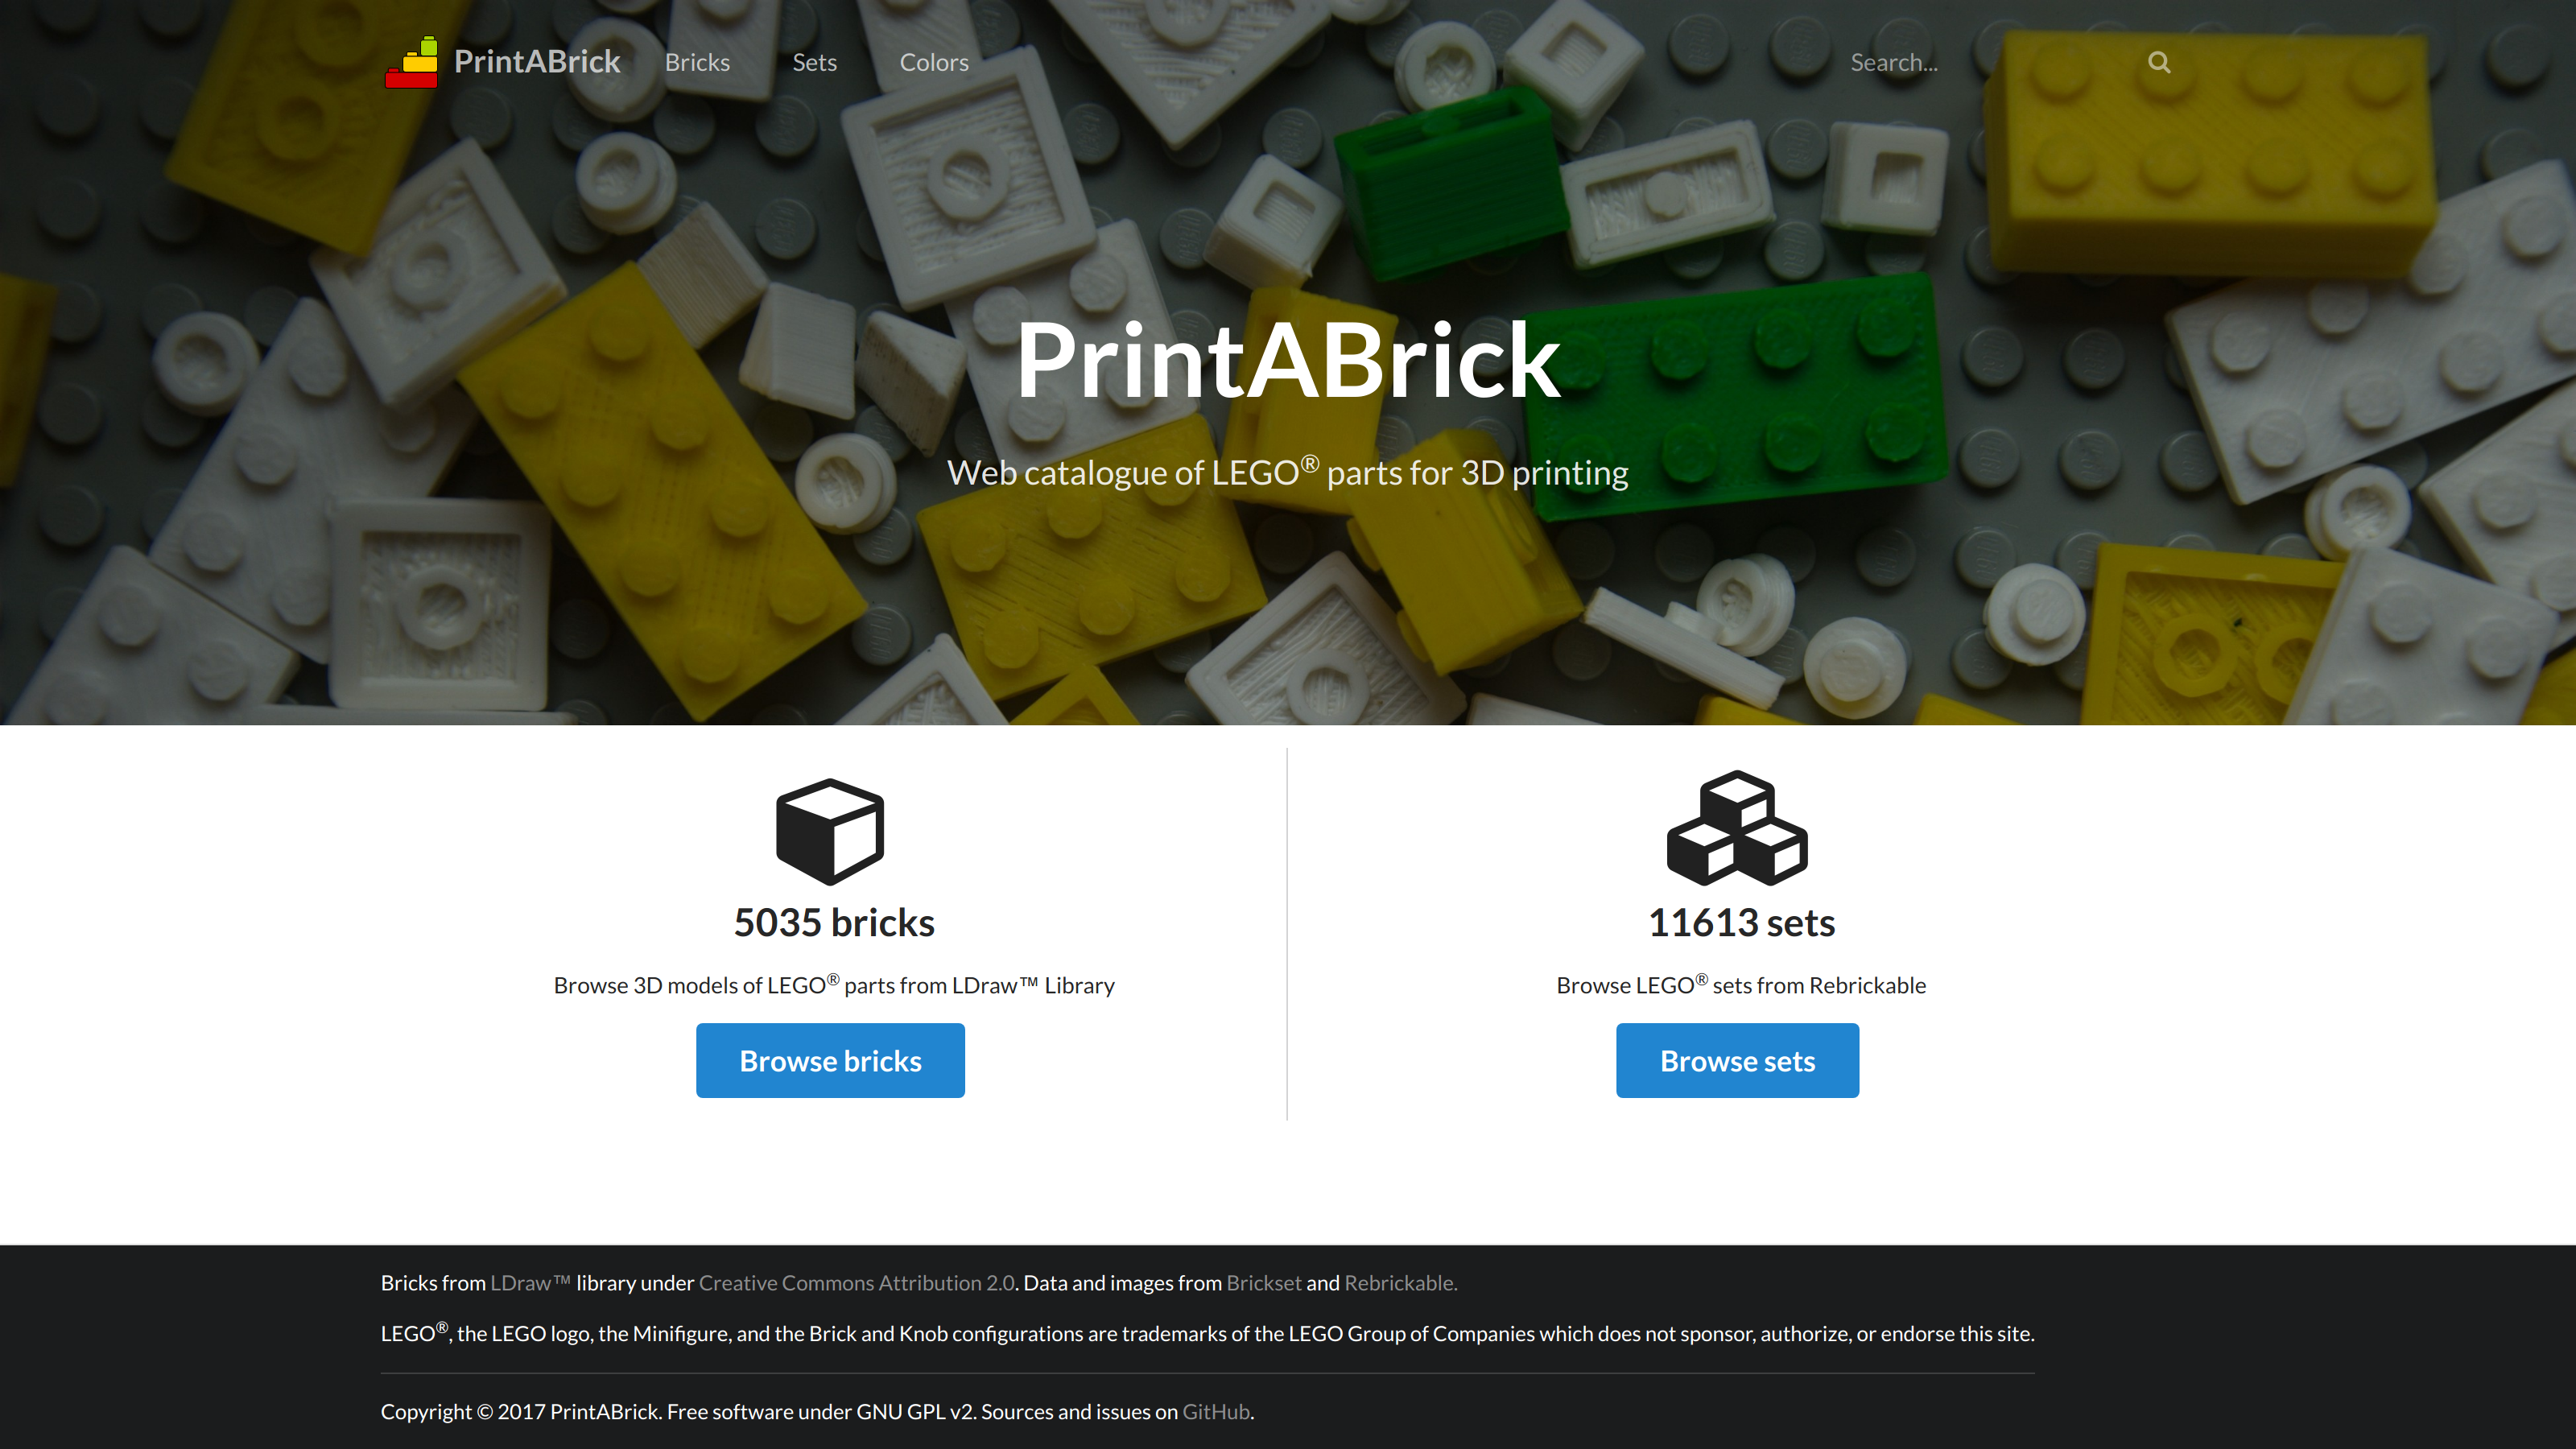
\includegraphics[width=\textwidth,height=\textheight,keepaspectratio]{images/screenshot-homepage.png}
    \caption{Snímek obrazovky - domovská stránka\label{facebook-share}}
\end{figure}

\begin{figure}[htbp]
    \centering
    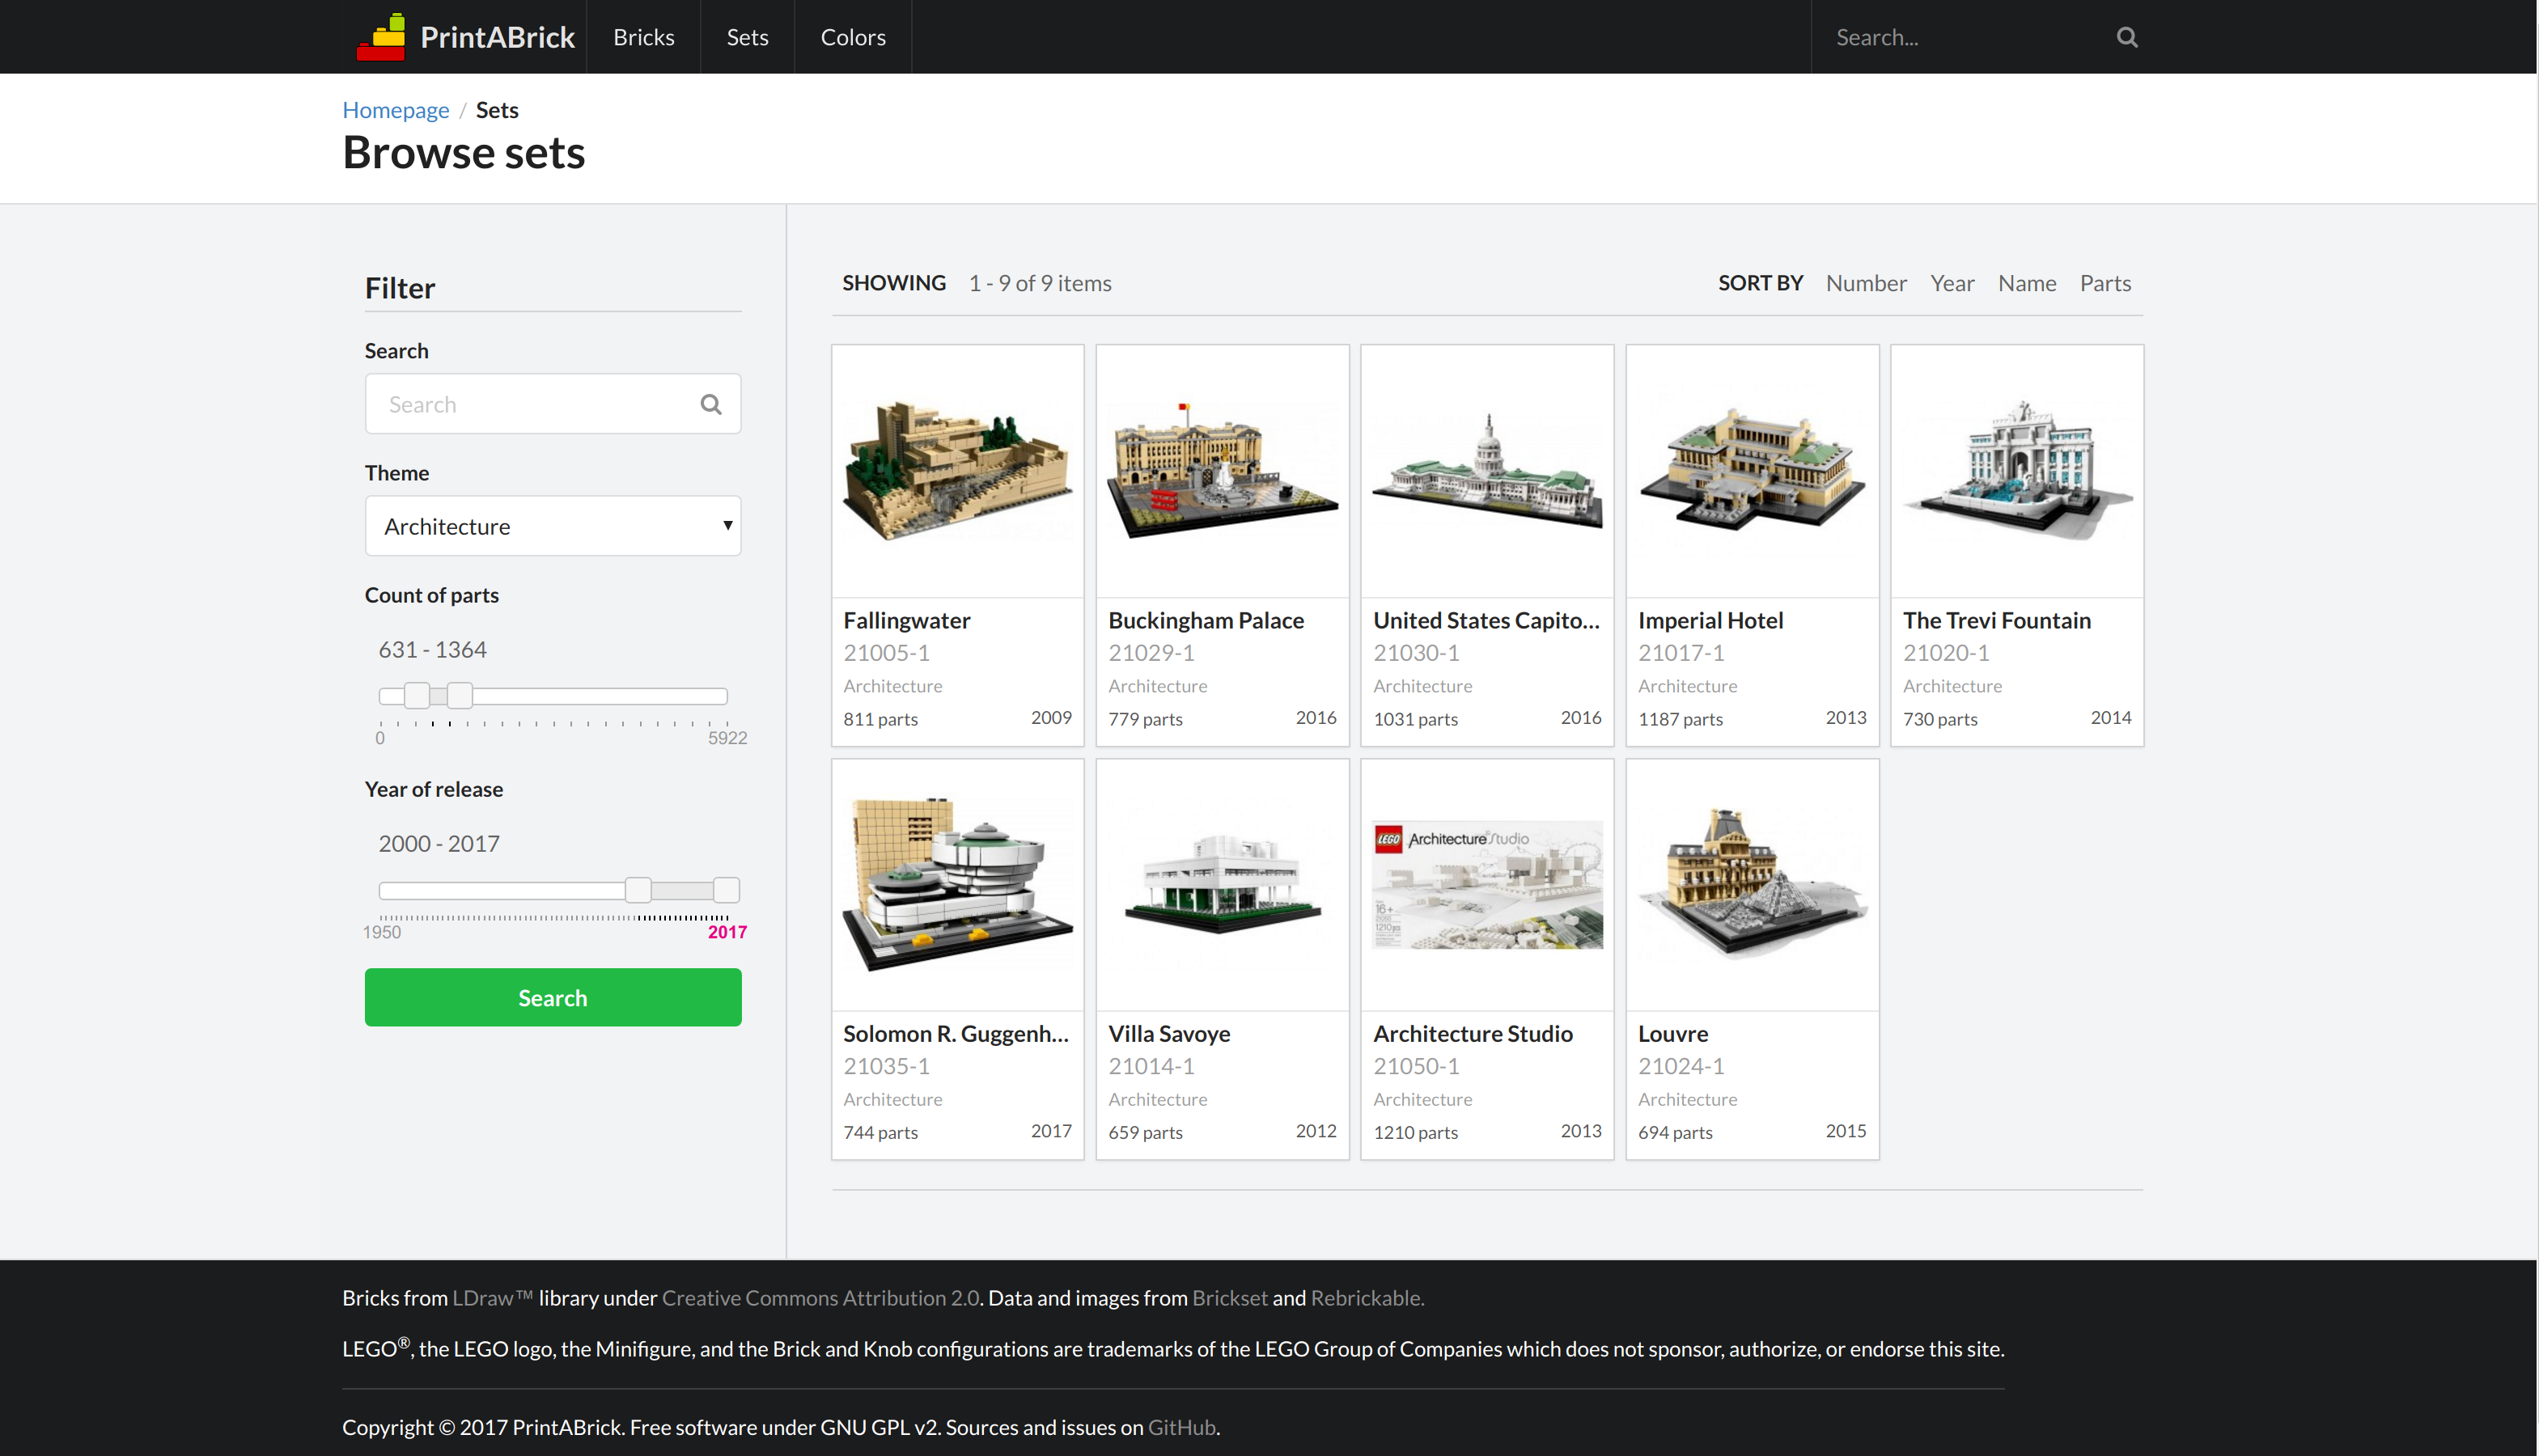
\includegraphics[width=\textwidth,height=\textheight,keepaspectratio]{images/screenshot-sets.png}
    \caption{Snímek obrazovky - výpis stavebnic\label{facebook-share}}
\end{figure}

\subsubsection*{Možnosti dalšího rozvoje}\label{moznosti-dalsiho-rozvoje}

V rámci možností dalšího rozvoje aplikace vidím následující:
\begin{itemize}
    \item výpočet odhadu množství materiálu potřebného k tisku,
    \item implementace správy sbírek 
\end{itemize} 

\label{conclusion}

\end{conclusion}

\printbibliography[title={Zdroje}]

\appendix

\chapter{Seznam použitých zkratek}
\printglossary[type=\acronymtype,style=acronyms]

\chapter{Instalační příručka}\label{append:instalace}
Tato instalační příručka je dostupná také v~anglické verzi v~podobě README.md souboru v~přiloženém zdrojovém kódu aplikace.

\section*{PrintABrick}\label{printabrick}

Webový katalog LEGO® dílů k~3D tisku

\subsubsection*{Systémové požadavky}\label{system-requirements}

\begin{itemize}
\tightlist
\item
  PHP verze 7.0 nebo vyšší
\item
  PHP rozšíření

  \begin{itemize}
  \tightlist
  \item
    FTP
  \item
    SOAP
  \item
    GD
  \item
    PDO
  \item
    Zip
  \end{itemize}
\item
  \emph{date.timezone} nastaveno v~souboru \emph{php.ini}
\end{itemize}

Zda váš systém splňuje minimální požadavky Symfony můžete zjistit příkazem \\\mintinline{console}{$ bin/symfony_requirements}

Pro kompletní požadavky navštivte Symfony 3.3 dokumentaci \autocite{symfony:requirements}.

\paragraph{Závislosti}

\begin{itemize}
\item
  Elasticsearch \textgreater{}= 5 \autocite{elasticsearch}
\item
  POV-Ray \autocite{povray}
\item
  stl2pov \autocite{stl2pov}
\item
  ADMesh
\item
  LDView OSMesa \textgreater{}= 4.2.1 \autocite{ldview}
\end{itemize}

\subsubsection*{Instalace}\label{installing}

\paragraph{Backend}

\begin{enumerate}
\def\labelenumi{\arabic{enumi}.}
\tightlist
\item
  Ujistěte se, že váš systém splňuje minimální požadavky.
\item
  Nainstalujte závislosti pomocí \href{https://getcomposer.org/}{Composer}, \mintinline{console}{$ composer install}.
\end{enumerate}

\paragraph{Frontend}

\begin{enumerate}
\def\labelenumi{\arabic{enumi}.}
\tightlist
\item
  Nainstalujte npm \autocite{npm} závislosti pomocí \mintinline{console}{$ npm install}.
\item
  Nainstalujte bower \autocite{bower} závislosti pomocí \mintinline{console}{$ bower install}.
\item
  Zkompilujte zdroje \mintinline{console}{$ gulp default [--env production]}.
\end{enumerate}

\paragraph{Inicializace}\label{initialization}

\subsubsection*{Nastavení databáze}\label{setup-database}

\begin{enumerate}
\def\labelenumi{\arabic{enumi}.}
\tightlist
\item
  Nastavte parametry aplikace v~souboru \\\mintinline{console}{app/config/parameters.yml}.
\item
  Vygenerujte prázdnou databázi příkazem \\\mintinline{console}{$ bin/console doctrine:database:create}.
\item
  Vytvořte tabulky databáze přikazem \\\mintinline{console}{$ bin/console doctrine:schema:create}.
\item
  Načtěte výchozí data do databáze \\\mintinline{console}{$ bin/console doctrine:fixtures:load}.
\end{enumerate}

\subsubsection*{Načtení dat}\label{load-data}

Kompletní inicializace dat aplikace může být provedena příkazem \\\mintinline{console}{$ bin/console app:init}.

Tento příkaz se skládá z~několika podpříkazů, které mohou být spuštěny samostatně:

\begin{enumerate}
\def\labelenumi{\arabic{enumi}.}
\tightlist
\item
Načtení součástek knihovny LDraw \\\mintinline{console}{$ bin/console app:load:ldraw [--ldraw=PATH] [--all] [--file=FILE] [--update]}.
\item
Načtení databáze Rebrickable \\\mintinline{console}{$ bin/console app:load:rebrickable}.
\item
Spárování součástek knihovny LDraw a databáze Rebrickable \\\mintinline{console}{$ bin/console app:load:relations}.
\item
Stažení/vykreslení obrázků součástek \\\mintinline{console}{$ bin/console app:load:images [--color=INT] [--rebrickable] [--missing]}.
\item
Zaindexování Elasticsearch \mintinline{console}{$ bin/console fos:elastica:populate}.
\end{enumerate}

\subsubsection*{Spustění aplikace na lokálním webserveru}
Aplikaci můžete spustit na lokálním PHP web serveru příkazem \mintinline{console}{$ bin/console server:start}.

\subsubsection*{Párování součástek}\label{adding-part-relation}

Vazby mezi součástkami z~knihovny LDraw a součástkami z~databáze Rebrickable jsou automaticky spárováný při běhu příkazu \\\mintinline{console}{$ bin/console app:load:relations}.

Vazby mezi součástkami, které nebyly automaticky rozpoznány je možné opravit přidáním odpovídajících ID do souboru \\\mintinline{console}{app/Resources/relations/part_model.yml}.

\subsection*{Testování}\label{testing}

Testy využívají zvláštní databázi, která musí být před prvním spuštěním testů vytvořena. Vytvoření testovací databáze:

\begin{enumerate}
\def\labelenumi{\arabic{enumi}.}
\tightlist
\item
  Vygenerujte prázdnou databázi příkazem \\\mintinline{console}{$ bin/console doctrine:database:create --env=test}.
\item
  Vytvořte tabulky databáze přikazem \\\mintinline{console}{$ bin/console doctrine:schema:create --env=test}.
\end{enumerate}

Kompletní systémové testy mohou být spučtěny příkazem \mintinline{console}{$ phpunit}.

Tyto testy pokrývají základní funkcionalitu aplikace, včetně testování úspěšnosti volání programů třetích stran,využívaných aplikací.

\chapter{Obsah přiloženého média}
\begin{figure}
	\dirtree{%
		.1 README.md\DTcomment{stručný popis obsahu média}.
		.1 src\DTcomment{zdrojové kódy implementace}.
		.1 thesis\DTcomment{text práce}.
			.2 latex\DTcomment{zdrojová forma práce ve formátu \XeLaTeX{}}.
			.2 BP\_Hubner\_David\_2017.pdf\DTcomment{text práce ve formátu PDF}.
	}
\end{figure}

\end{document}